%%%%%%%%%%%%%%%%%%%%%%%%%%%%%%%%%%%%%%%%%
% Beamer Presentation
% LaTeX Template
% Version 1.0 (10/11/12)
%
% This template has been downloaded from:
% http://www.LaTeXTemplates.com
%
% License:
% CC BY-NC-SA 3.0 (http://creativecommons.org/licenses/by-nc-sa/3.0/)
%
%%%%%%%%%%%%%%%%%%%%%%%%%%%%%%%%%%%%%%%%%

%----------------------------------------------------------------------------------------
%	PACKAGES AND THEMES
%----------------------------------------------------------------------------------------

\documentclass{Bredelebeamer}
\usefonttheme[onlymath]{serif}
\mode<presentation> {

% The Beamer class comes with a number of default slide themes
% which change the colors and layouts of slides. Below this is a list
% of all the themes, uncomment each in turn to see what they look like.

%\usetheme{default}
%\usetheme{AnnArbor}
%\usetheme{Antibes}
%\usetheme{Bergen}
%\usetheme{Berkeley}
%\usetheme{Berlin}
%\usetheme{Boadilla}
%\usetheme{CambridgeUS}
%\usetheme{Copenhagen}
%\usetheme{Darmstadt}
%\usetheme{Dresden}
%\usetheme{Frankfurt}
%\usetheme{Goettingen}
%\usetheme{Hannover}
%\usetheme{Ilmenau}
%\usetheme{JuanLesPins}
%\usetheme{Luebeck}
\usetheme{Madrid}
%\usetheme{Malmoe}
%\usetheme{Marburg}
%\usetheme{Montpellier}
%\usetheme{PaloAlto}
%\usetheme{Pittsburgh}
%\usetheme{Rochester}
%\usetheme{Singapore}
%\usetheme{Szeged}
%\usetheme{Warsaw}

% As well as themes, the Beamer class has a number of color themes
% for any slide theme. Uncomment each of these in turn to see how it
% changes the colors of your current slide theme.

%\usecolortheme{albatross}
%\usecolortheme{beaver}
%\usecolortheme{beetle}
%\usecolortheme{crane}
%\usecolortheme{dolphin}
%\usecolortheme{dove} %\usecolortheme{fly}
%\usecolortheme{lily}
%\usecolortheme{orchid}
%\usecolortheme{rose}
%\usecolortheme{seagull}
%\usecolortheme{seahorse}
%\usecolortheme{whale}
%\usecolortheme{wolverine}

%\setbeamertemplate{footline} % To remove the footer line in all slides uncomment this line
%\setbeamertemplate{footline}[page number] % To replace the footer line in all slides with a simple slide count uncomment this line

%\setbeamertemplate{navigation symbols}{} % To remove the navigation symbols from the bottom of all slides uncomment this line
}

\usepackage{graphicx} % Allows including images
\usepackage{booktabs} % Allows the use of \toprule, \midrule and \bottomrule in tables
\usepackage{amssymb}
\usepackage{amsmath}
\usepackage{mathtools}
\usepackage{pdfpages}
\usepackage{eso-pic}
\usepackage{bm}
\usepackage[utf8]{inputenc}


%----------------------------------------------------------------------------------------
%	TITLE PAGE
%----------------------------------------------------------------------------------------

\title[GAN]{Generative Adversarial Networks} % The short title appears at the bottom of every slide, the full title is only on the title page

\author{Bruno Gavranović} % Your name
\institute[PSIML2017] % Your institution as it will appear on the bottom of every slide, may be shorthand to save space
{
Petnica Summer School of Machine Learning\\ % Your institution for the title page
\medskip
\textit{bruno.gavranovic@fer.hr} % Your email address
}
\date{\today} % Date, can be changed to a custom date
\graphicspath{{img/}}

\begin{document}

\begin{frame}
	\begin{figure}[h!]
		\centering
		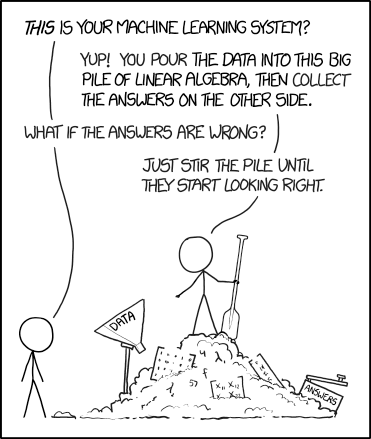
\includegraphics[height=0.9\textheight]{xkcd_ml.png}
	\end{figure}
\end{frame}

\begin{frame}
\titlepage % Print the title page as the first slide
\end{frame}

\begin{frame}
\frametitle{Overview} % Table of contents slide, comment this block out to remove it
\tableofcontents % Throughout your presentation, if you choose to use \section{} and \subsection{} commands, these will automatically be printed on this slide as an overview of your presentation
\end{frame}

%----------------------------------------------------------------------------------------
%	PRESENTATION SLIDES
%----------------------------------------------------------------------------------------

%------------------------------------------------
\section{Meta} % Sections can be created in order to organize your presentation into discrete blocks, all sections and subsections are automatically printed in the table of contents as an overview of the talk
%------------------------------------------------

\begin{frame} \frametitle{Meta}
\begin{itemize}[<+->]
	\item What is this talk about?
	\item New idea
\end{itemize}

\pause[3]
\begin{block}{Yann LeCun}
"The most important one, in my opinion, is adversarial training (also called GAN for Generative Adversarial Networks).

This, and the variations that are now being proposed is the most interesting idea in the last 10 years in ML, in my opinion.”
\end{block}

\begin{itemize}[<+(1)->]
	\item Nobody is still sure how it works
	\item Compared to other ML models, we're still in early stages
	\item Our understanding of it changes from week to week
\end{itemize}
\end{frame}

%------------------------------------------------

\begin{frame}
\begin{figure}[h!]
	\centering
	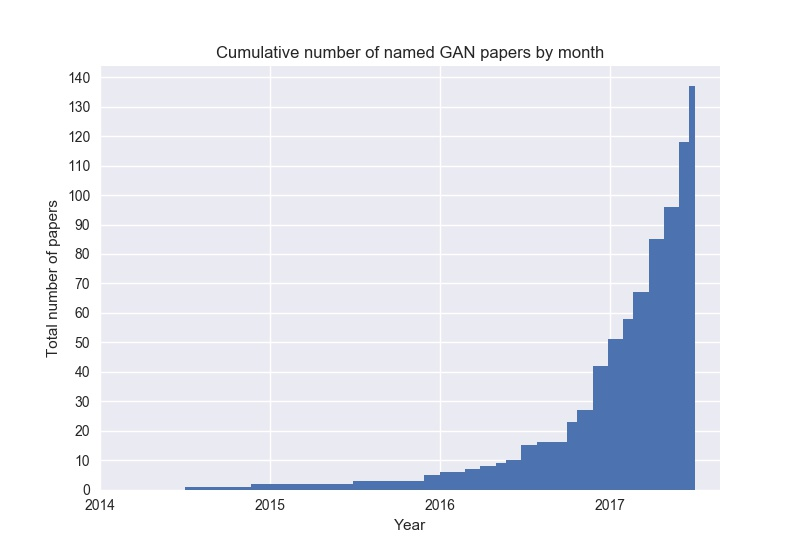
\includegraphics[width=\textwidth]{gan_timeline.jpg}
\end{figure}

\end{frame}

%------------------------------------------------

\begin{frame}
	\frametitle{GAN: Just tell me what it is}
	\begin{itemize}
		\item Generative machine learning model in which two neural networks are competing against each other
	\end{itemize}
\begin{figure}[h!]
	\centering
	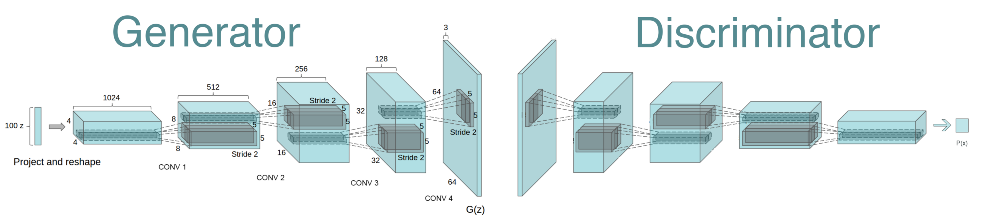
\includegraphics[width=\textwidth]{dcgan_both.png}
\end{figure}
	\pause
	\begin{itemize}[<+->]
		\item Instead of using a standard fixed cost function, we \textit{learn} the cost function with the neural network
		\item We alternate between training different parts of the network
		\item Forger and the police
		\item It's difficult to train and analyze
	\end{itemize}
\footnotetext{\url{https://github.com/dmonn/GAN-face-generator}}
\end{frame}

\begin{frame}
\begin{figure}[h!]
	\centering
	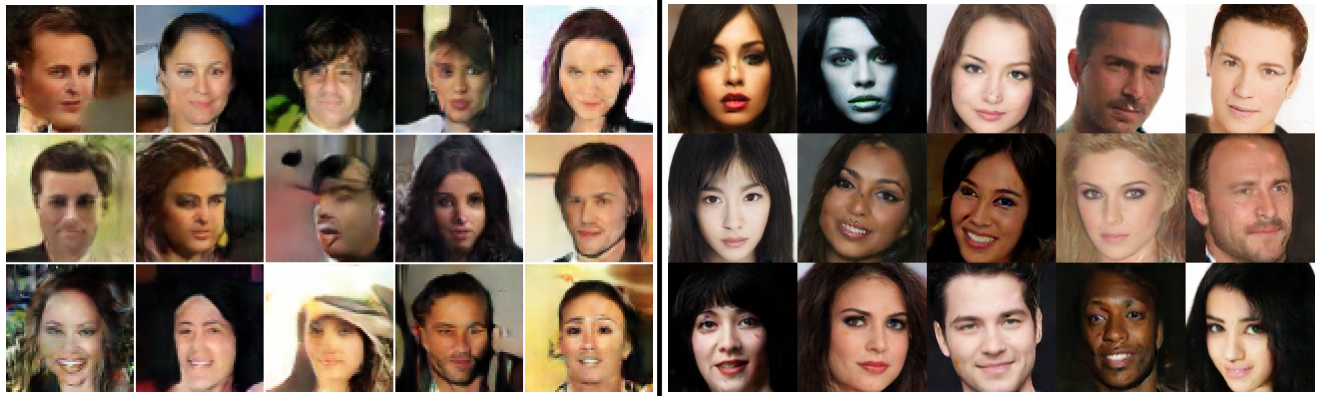
\includegraphics[width=\textwidth]{which_is_real.png}
	\caption{Which side are real images?}
	\label{fig:which_is_real}
\end{figure}
\end{frame}


%------------------------------------------------
\begin{frame}
\begin{figure}[h!]
	\centering
	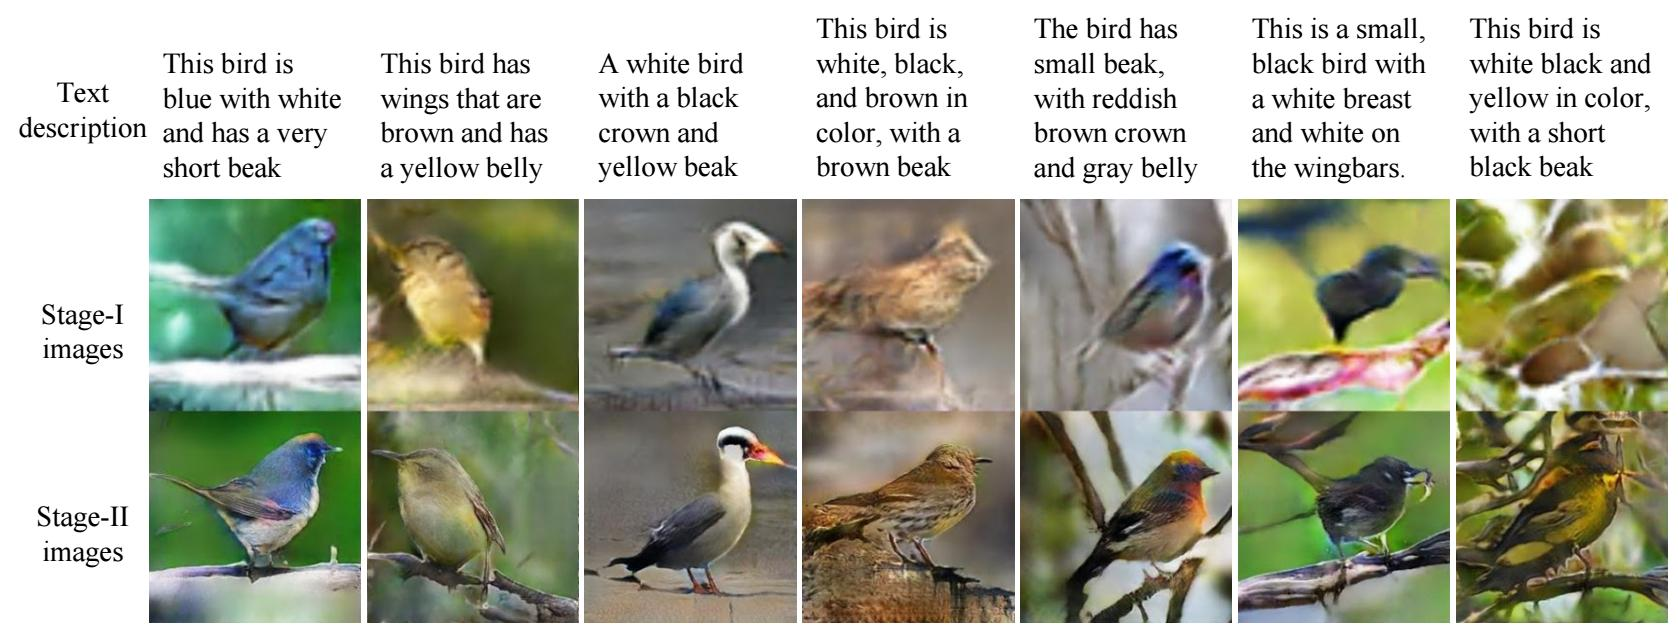
\includegraphics[width=\textwidth]{stack_gan.jpg}
	\caption{StackGAN}
\end{figure}
\end{frame}

\begin{frame}
\begin{figure}[h!]
	\centering
	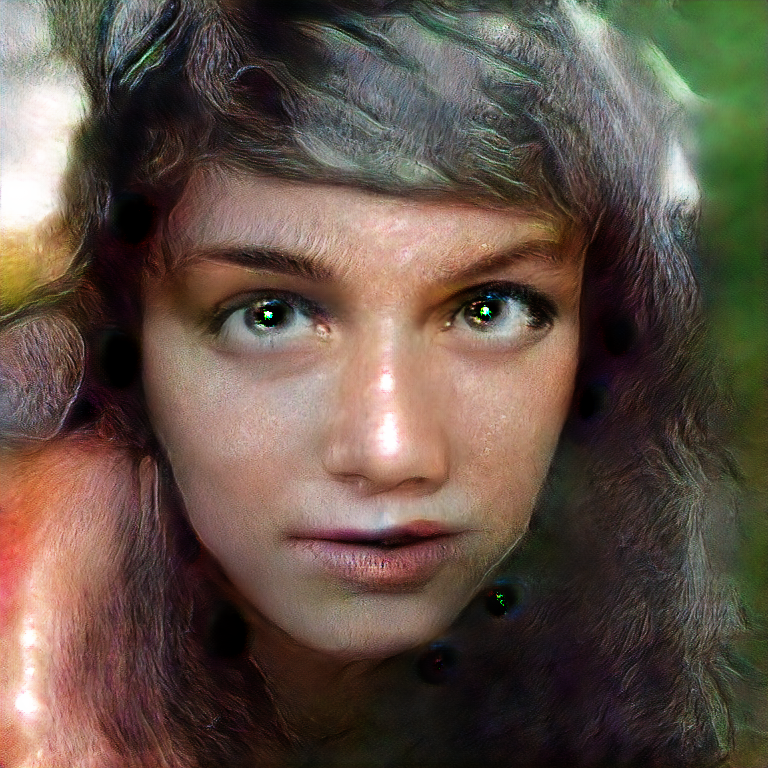
\includegraphics[width=0.8\textwidth]{4k_woman.jpg}
\end{figure}
\end{frame}

\begin{frame}
\begin{figure}[h!]
	\centering
	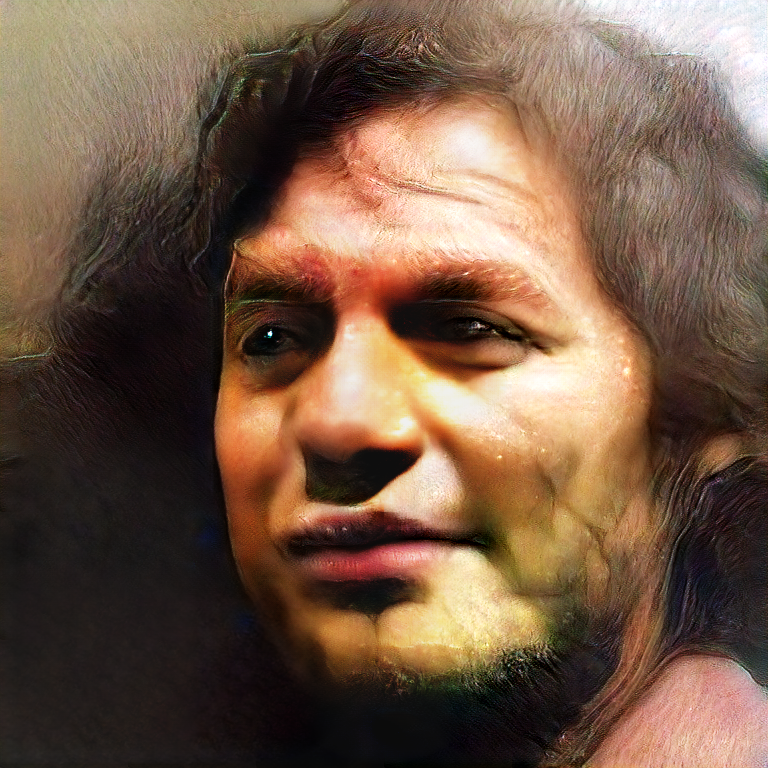
\includegraphics[width=0.8\textwidth]{4k_man.jpg}
\end{figure}
\end{frame}

\begin{frame}
\begin{figure}[h!]
	\centering
	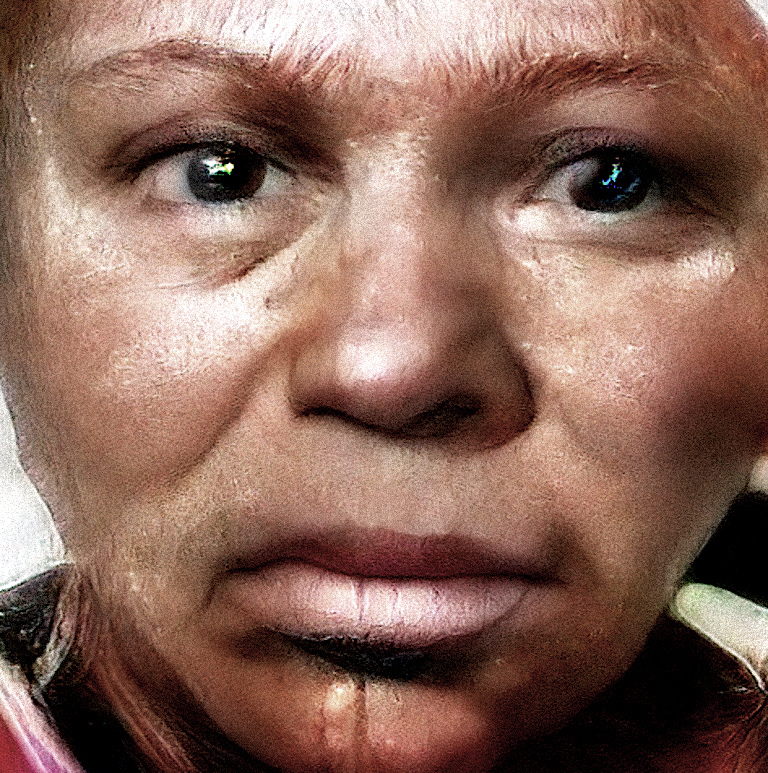
\includegraphics[width=0.8\textwidth]{4k_black_woman.jpg}
\end{figure}
\end{frame}
%------------------------------------------------
\begin{frame}
\frametitle{What is this talk about?}
\begin{itemize}
	\item Theory behind Generative Adversarial Networks
	\item Comparison of different models
	\item Practical advice for training
	\item Everything is a Work In Progress.
\end{itemize}

\end{frame}


\section{Prerequisites}
\subsection{The manifold hypothesis}


\begin{frame}
\frametitle{Prerequisites}
\begin{figure}[h!]
	\centering
	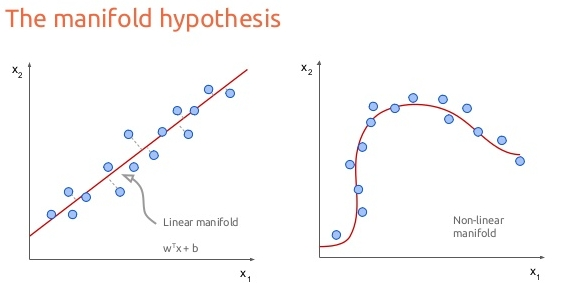
\includegraphics[width=0.8\textwidth]{manifold_hypothesis.jpg}
\end{figure}
\begin{itemize}[<+(1)->]
	\item Understanding real world data
	\item Natural data forms a low dimensional manifold in its embedding space
\end{itemize}

\end{frame}
\begin{frame}
\begin{figure}[h!]
	\centering
	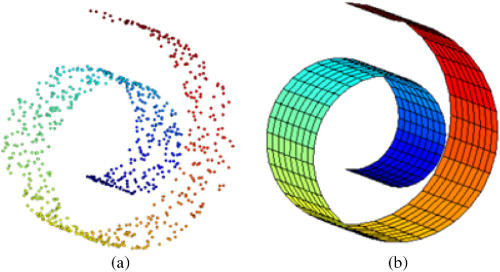
\includegraphics[width=0.8\textwidth]{swiss_roll.jpg}
\end{figure}

\end{frame}

\begin{frame}
\begin{figure}[h!]
	\centering
	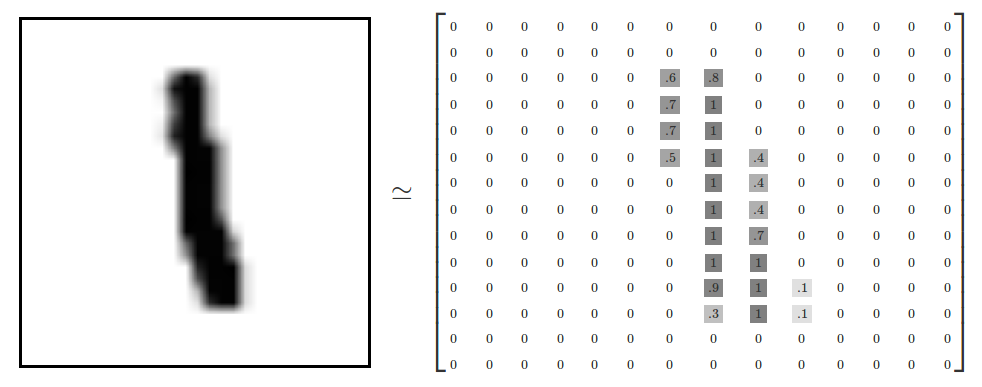
\includegraphics[width=\textwidth]{mnist_pixel_space.png}
\end{figure}

\end{frame}

\begin{frame}
\begin{figure}[h!]
	\centering
	\includegraphics<1>[width=\textwidth]{distr/1.png}
	\includegraphics<2>[width=\textwidth]{distr/2.png}
	\includegraphics<3>[width=\textwidth]{distr/3.png}
	\includegraphics<4>[width=\textwidth]{distr/4.png}
	\includegraphics<5>[width=\textwidth]{distr/5.png}
	\includegraphics<6>[width=\textwidth]{distr/6.png}
	\includegraphics<7->[width=\textwidth]{distr/7.png}
\end{figure}
\begin{itemize}[<+(6)->]
	\item We have a random vector $ \bm{z} \sim \mathcal{Z}$
		\item We can define a parametric function $g_\theta: \mathcal{Z} \rightarrow \mathcal{X}$ that generates samples from a certain distribution $\mathbb{P}_\theta$
		\item We have samples from the real data distribution $\mathbb{P}_\textit{r}$
		\item By varying $\theta$ we can make the $\mathbb{P}_\theta$ distribution arbitrarily close to $\mathbb{P}_\textit{r}$
		\item How do we define ``close"?
\end{itemize}
\end{frame} 

%------------------------------------------------

\section{Comparison with autoencoders}

\begin{frame}
\frametitle{First attempt}
\begin{columns}
\begin{column}{0.5\textwidth}
	\begin{itemize}[<+->]
		\item How to match the distributions?
		\item Autoencoder as an example
		\item Network decomposition into basic building blocks
		\item Tools for thinking about neural networks
	\end{itemize}
\end{column}
\begin{column}{0.5\textwidth}  
	\begin{figure}[h!]
		\centering
		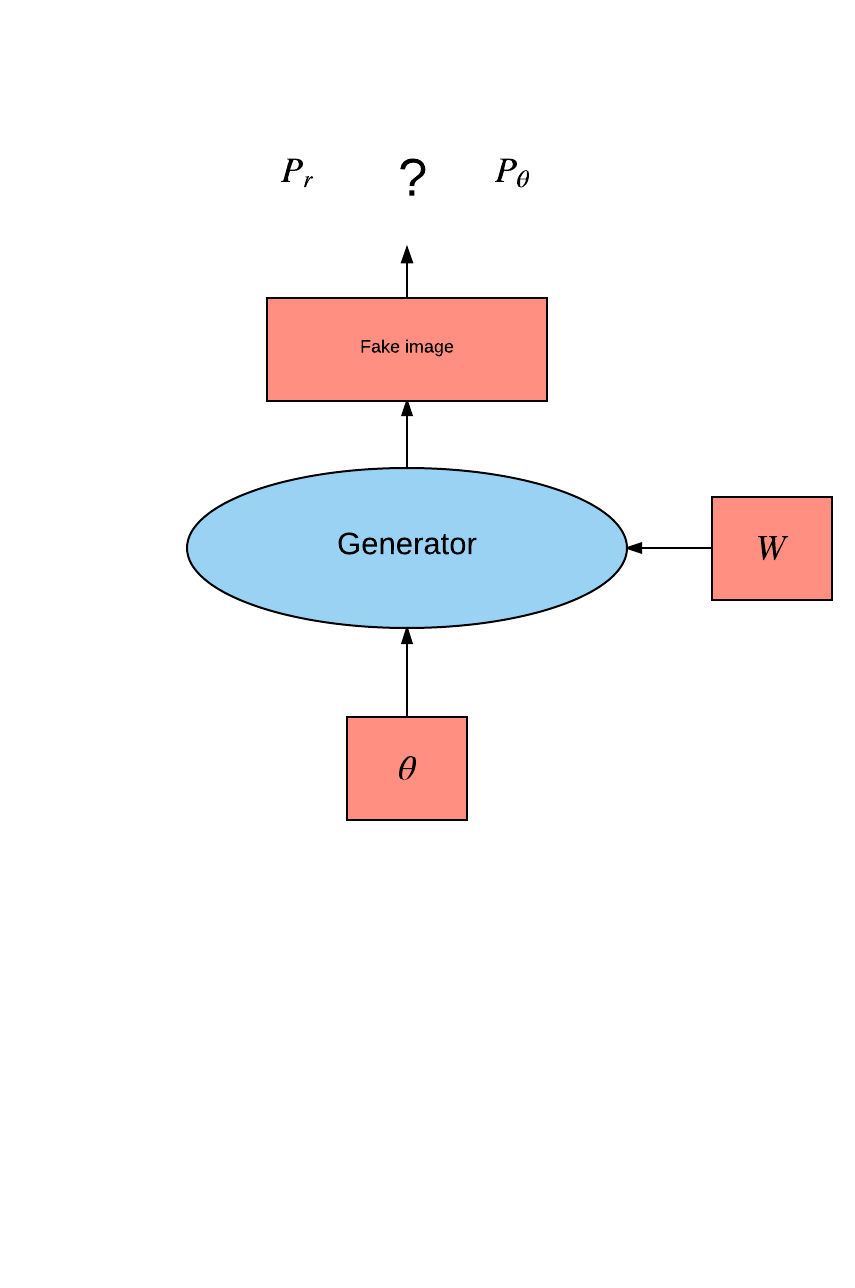
\includegraphics[width=0.8\textwidth]{first_attempt_gan.png}
	\end{figure}
\end{column}
\end{columns}


\end{frame}

%------------------------------------------------

\begin{frame}
\frametitle{Autoencoder}
\begin{columns}
\begin{column}{0.5\textwidth}
\begin{itemize}
	\item Recreation of samples from the real distribution
	\item Encoding the images into the bottleneck $\theta$
	\item Implicitly training the network to extract useful features
\end{itemize}
\end{column}
\begin{column}{0.5\textwidth}
\begin{figure}[h!]
	\centering
	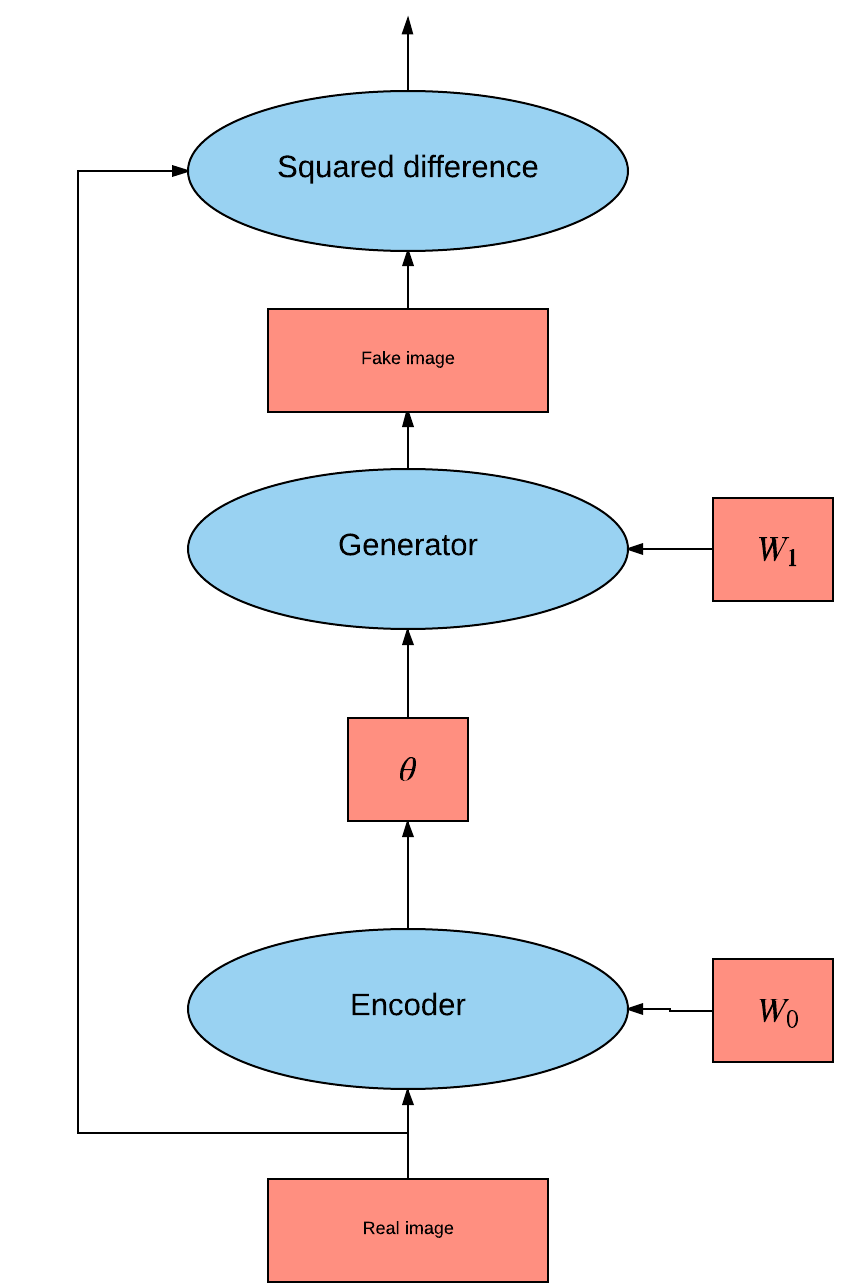
\includegraphics[width=0.8\textwidth]{autoencoder_attempt.png}
\end{figure}
\end{column}
\end{columns}

\end{frame}
\subsection{Computational graph perspective}

%------------------------------------------------
\begin{frame}
	\begin{columns}
	\begin{column}{0.3\textwidth}
		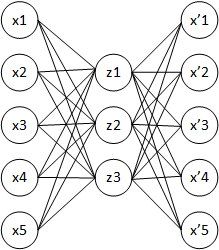
\includegraphics[width=\textwidth]{autoencoder_bad_diagram.png}
	\end{column}
	\pause
	\begin{column}{0.33\textwidth}
		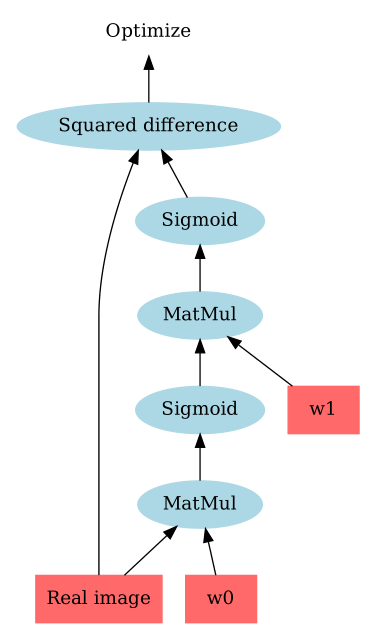
\includegraphics[width=\textwidth]{sq_diff.png}
	\end{column}
	\pause
	\begin{column}{0.34\textwidth}
		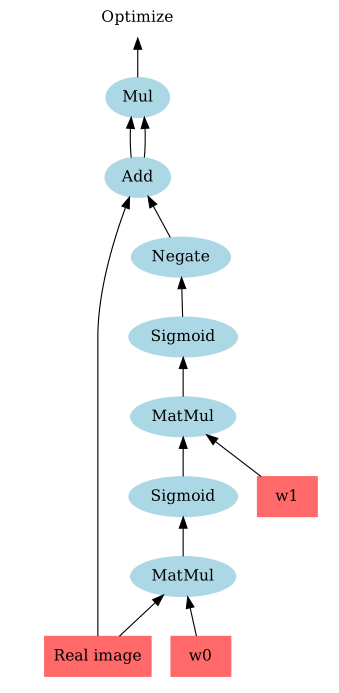
\includegraphics[width=0.8\textwidth]{sq_diff_all.png}
	\end{column}
	\end{columns}
	\pause[4]
	\begin{block}{Things to note}
	\begin{enumerate}
		\item Cost function is not parametrized (it's fixed)
		\item We train the network with just one cost function
		\item Weight freezing and sharing is fixed throughout the training
	\end{enumerate}
	\end{block}
\end{frame}
%------------------------------------------------
\begin{frame}
	\frametitle{Cost function}
	\begin{itemize}
		\item MSE needs to average over all possibilities and choose a single answer
		\item Square error - a simple parabola, is it sufficient?
	\end{itemize}
	\begin{figure}[h!]
		\centering
		\includegraphics<1>[width=\textwidth]{predict_frame.png}
		\includegraphics<2->[width=\textwidth]{mse_vs_adversarial.png}
	\end{figure}
	\footnotetext{Ian J. Goodfellow:
NIPS 2016 Tutorial: Generative Adversarial Networks}
\end{frame}

%------------------------------------------------
\begin{frame}
	\begin{figure}[h!]
	\centering
	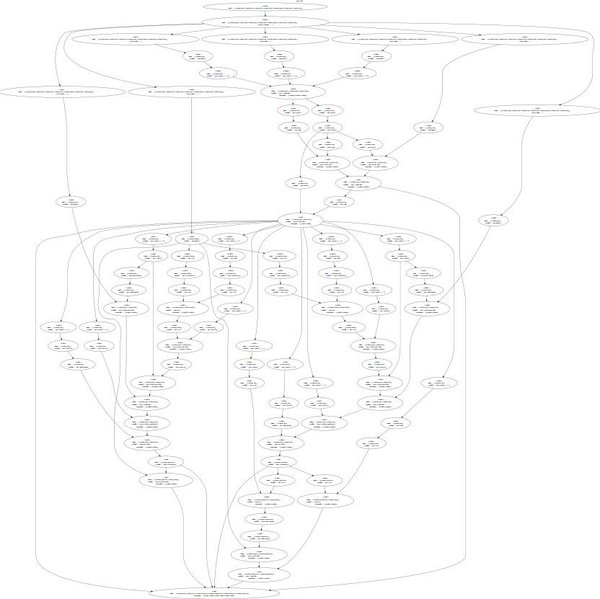
\includegraphics[width=0.6\textwidth]{ntm_comp_graph.jpg}
	\caption{Neural turing machines computational graph}
	\label{fig:ntm_comp_graph}
	\end{figure}

\end{frame}
%------------------------------------------------
\begin{frame}
	\frametitle{The great idea}
	\begin{itemize}[<+->]
		\item Neural network is a computational graph!
		\item Cost function \textit{is a part of} that computational graph
		\item The great idea - why don't we put a neural network as the cost function?
		\item Introduces a lot of problems
		\item How do we even train this thing?
		\item How do we analyze it's behaviour?
		\item Partial answer to the "How do we know it's close?" question from the beginning
	\end{itemize}
\end{frame}

\subsection{Training regime}
%------------------------------------------------
\begin{frame}
	\frametitle{Training regime}
	\begin{figure}[h!]
	\centering
	\includegraphics<1>[width=\textwidth]{gan_optimization/GAN_optimization_1.png}
	\includegraphics<2>[width=\textwidth]{gan_optimization/GAN_optimization_2.png}
	\includegraphics<3>[width=\textwidth]{gan_optimization/GAN_optimization_3.png}
	\includegraphics<4>[width=\textwidth]{gan_optimization/GAN_optimization_4.png}
	\includegraphics<5>[width=\textwidth]{gan_optimization/GAN_optimization_5.png}
	\includegraphics<6->[width=\textwidth]{gan_optimization/GAN_optimization_6.png}
	\end{figure}
	\pause[6]
	\begin{itemize}
		\item Two-step optimization optimization process
	\end{itemize}
\end{frame}

%------------------------------------------------
\begin{frame}
	\frametitle{Intuitive approach}
	\begin{itemize}[<+->]
		\item Forger and the police
		\item Forger tries to create real looking money
		\item Police tries to get better at detecting fake money
		\item They both keep improving until the difference between fake and real money is imperceptible to us
	\end{itemize}
\end{frame}

\section{Statistical distances}
\subsection{Comparison of various statistical distances}
%------------------------------------------------
\begin{frame}
	\frametitle{Different statistical distances}
	\begin{itemize}[<+->]
		\item Recall from before - we have real and fake images, we want the fake distribution to become the same as the real distribution
		\item Instead of comparing distributions in the pixel space - we use the neural network (the cost function) to transform them to a more suitable representation
		\item But we still have to compare those distributions
		\item Defining distance between two points in Euclidean space is intuitive
		\item How do we define distances between distributions?
	\end{itemize}
\end{frame}
%------------------------------------------------
\begin{frame}
	\frametitle{Various statistical distances - divergences}
	\begin{itemize}
		\item KL-divergence
		\item JS-divergence
		\item Earth-mover distance (Wasserstein distance)
		\item Total variation distance
		\item Hellinger distance
		\item Mahalanobis distance
		\item Bhattacharyya distance
		\item Energy distance
		\item ...
	\end{itemize}
\end{frame}
%------------------------------------------------
\begin{frame}
	\frametitle{Kullback-Leibler and Jensen Shannon divergence}
	\begin{exampleblock}{KL-divergence}
	\[
		KL(\mathbb{P} \vert \vert \mathbb{Q}) = \mathbb{E}_{x \sim \mathbb{P}} \left[ \log \frac{P(x)}{Q(x)} \right] \pause = \int_{x} \log \frac{P(x)}{Q(x)} P(x) dx
	\]
\end{exampleblock}
\pause
	\begin{itemize}[<+->]
		\item Doesn't satisfy triangle inequality and symmetry
		\item Origins in information theory
		\item Information gained when revising from prior Q to posterior P

	\end{itemize}
	\pause[6]
	\begin{exampleblock}{JS-divergence}
	\[
		\mathbb{M} &= \frac{1}{2}(\mathbb{P} + \mathbb{Q})
	\]
	\pause[7]
	\[
		JS(\mathbb{P} \vert \vert \mathbb{Q}) &= \frac{1}{2}KL(\mathbb{P} \vert \vert \mathbb{M}) + \frac{1}{2}KL(\mathbb{Q} \vert \vert \mathbb{M})
	\]
\end{exampleblock}
	\begin{itemize}[<+(1)->]
		\item Symmetric and bounded
		\item Original GAN paper minimizes JS-divergence
	\end{itemize}
\end{frame}

%------------------------------------------------
\begin{frame}
	\frametitle{Wasserstein (Earth mover) distance}
	\begin{exampleblock}{EM distance}
	\[
		W(\mathbb{P}, \mathbb{Q}) = \inf_{\gamma \in \Pi(\mathbb{P}, \mathbb{Q})} {\mathbb{E}_{(x, y) \sim \gamma}} \left[ \lvert \lvert x - y \lvert \lvert \right]
	\]
\end{exampleblock}
	\begin{itemize}[<+->]
		\item Distance function that takes into account underlying geometry of the distributions
		\item Minimum cost of turning a pile of dirt into the other
		\item Proposed by Arjovsky \textit{et al.} as improvement to original GAN training - Wasserstein GAN
		\item Intractable
	\end{itemize}
\end{frame}
\subsection{Comparison on toy example}
%------------------------------------------------
\begin{frame}
	\frametitle{Learning distributions - toy example}
	\begin{figure}[h!]
		\centering
		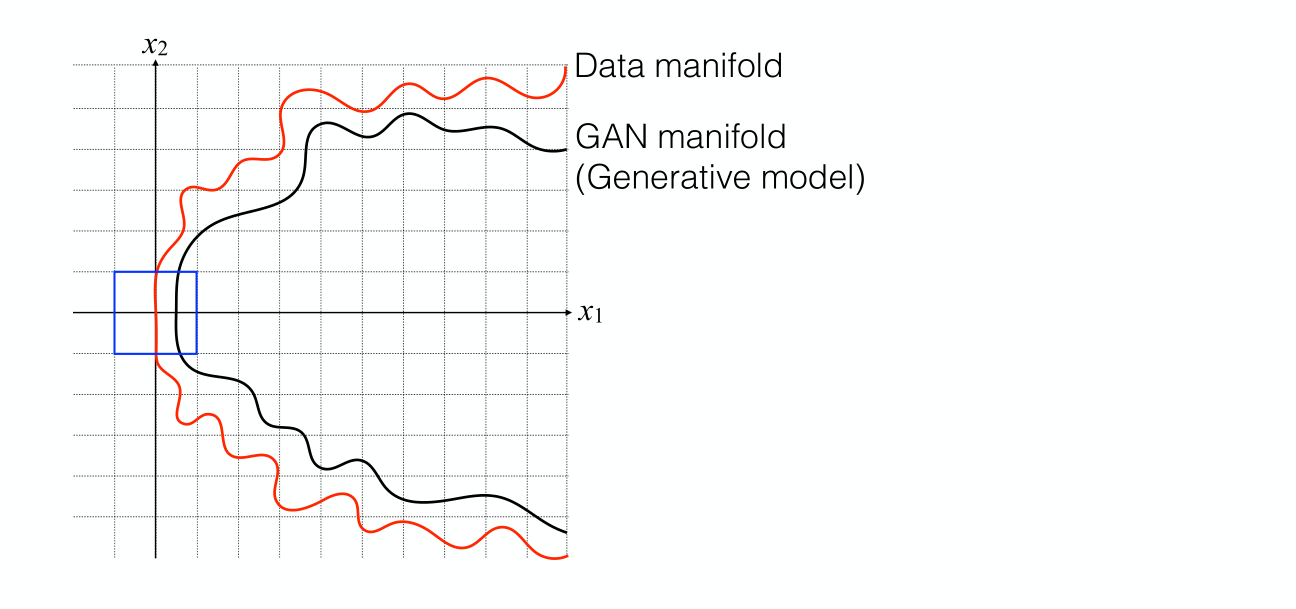
\includegraphics[width=\textwidth]{data_gan_manifold.png}
	\end{figure}
\footnotetext{MILA DLSS: \url{https://drive.google.com/file/d/0B_wzP_JlVFcKQ21udGpTSkh0aVk/view}}
\end{frame}

%------------------------------------------------

\begin{frame}
	\frametitle{Learning distributions - toy example}
	\begin{figure}[h!]
		\centering
		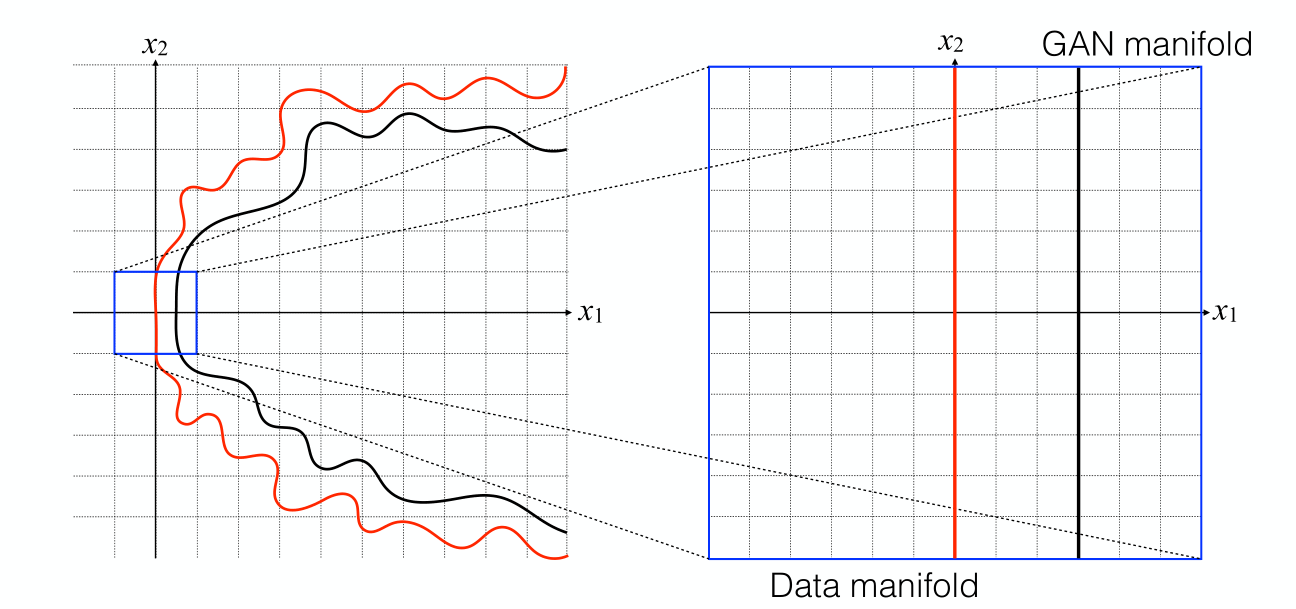
\includegraphics[width=\textwidth]{data_gan_manifold_zoom.png}
	\end{figure}
	\footnotetext{MILA DLSS: \url{https://drive.google.com/file/d/0B_wzP_JlVFcKQ21udGpTSkh0aVk/view}}
\end{frame}

%------------------------------------------------
\begin{frame}
	\frametitle{Learning distributions - toy example}
	\begin{columns}
	\begin{column}{0.5\textwidth}
	\begin{figure}[h!]
		\centering
		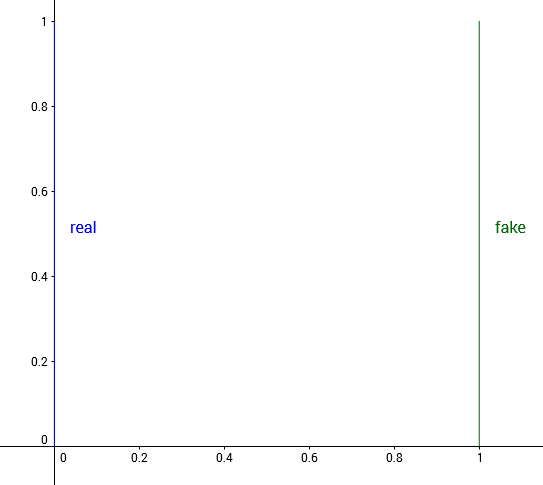
\includegraphics[width=0.9\textwidth]{two_lines.png}
	\end{figure}
	\pause
	$\mathbb{P}_r = (0, y) \quad \quad \quad \quad \quad \quad \mathbb{P}_g = (\theta, y)$
	\pause
	\begin{center}
		$y \sim U\big[0, 1\big]$
	\end{center}
	\end{column}
	\begin{column}{0.5\textwidth}  %%<--- here
	\pause
	\begin{itemize}
		\item Two distributions defined on $\mathbb{R}^2$
			\newline
		\pause
		\item  $ KL(\mathbb{P}_r \vert \vert \mathbb{P}_g) = +\infty$
		\pause
		\item  $ KL(\mathbb{P}_g \vert \vert \mathbb{P}_r) = +\infty$
		\pause
		\item  $ JS(\mathbb{P}_r, \mathbb{P}_g) = JS(\mathbb{P}_g, \mathbb{P}_r) = \log 2 $
		\pause
		\item  $ W(\mathbb{P}_r, \mathbb{P}_g) = W(\mathbb{P}_g, \mathbb{P}_r) = \vert \theta \vert $
	\end{itemize}
	\end{column}
	\end{columns}
	\footnotetext{\url{http://www.alexirpan.com/2017/02/22/wasserstein-gan.html}}
\end{frame}
%------------------------------------------------
\begin{frame}
	\frametitle{JS and EM distance w.r.t. $\theta$ }
	\begin{columns}
	\begin{column}{0.5\textwidth}
	\begin{figure}[h!]
		\centering
		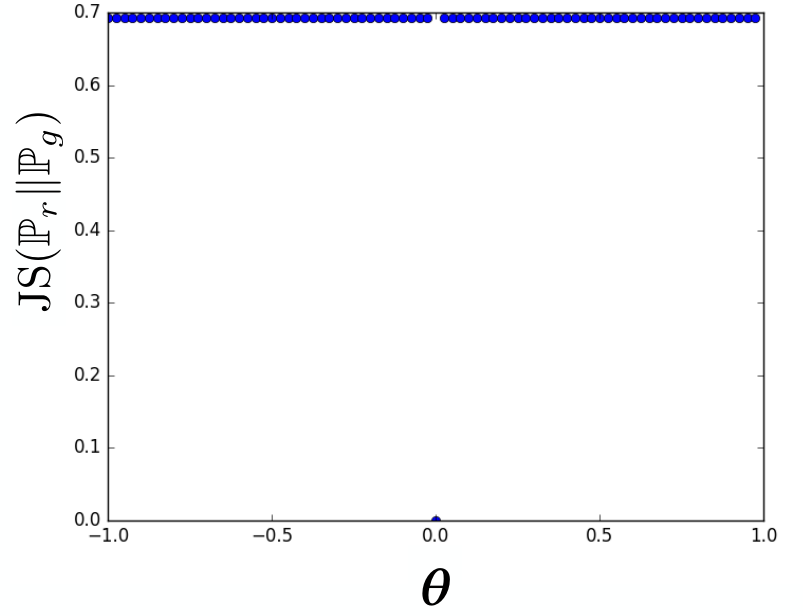
\includegraphics[width=\textwidth]{JS_value.png}
	\end{figure}
	\pause
	\begin{itemize}
		\item JS-divergence gradient is zero
	\end{itemize}
	\end{column}
	\begin{column}{0.5\textwidth}  %%<--- here
	\pause
	\begin{figure}[h!]
		\centering
		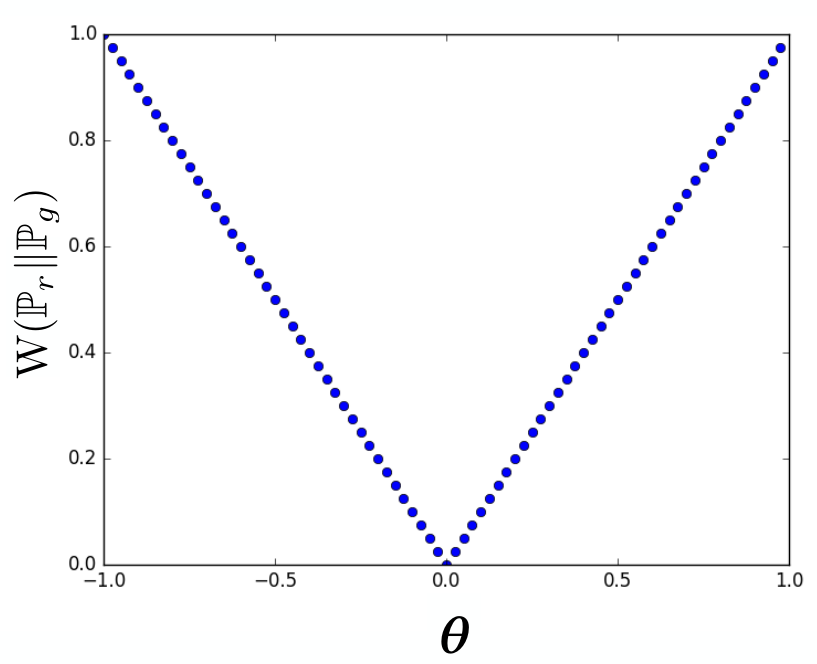
\includegraphics[width=\textwidth]{wasserstein_value.png}
	\end{figure}
	\pause
	\begin{itemize}
		\item Wasserstein gradient is constant
	\end{itemize}
	\end{column}
	\end{columns}
\end{frame}
%------------------------------------------------
\begin{frame}
	\frametitle{Gradients between two gaussian distributions}
	\begin{figure}[h!]
		\centering
		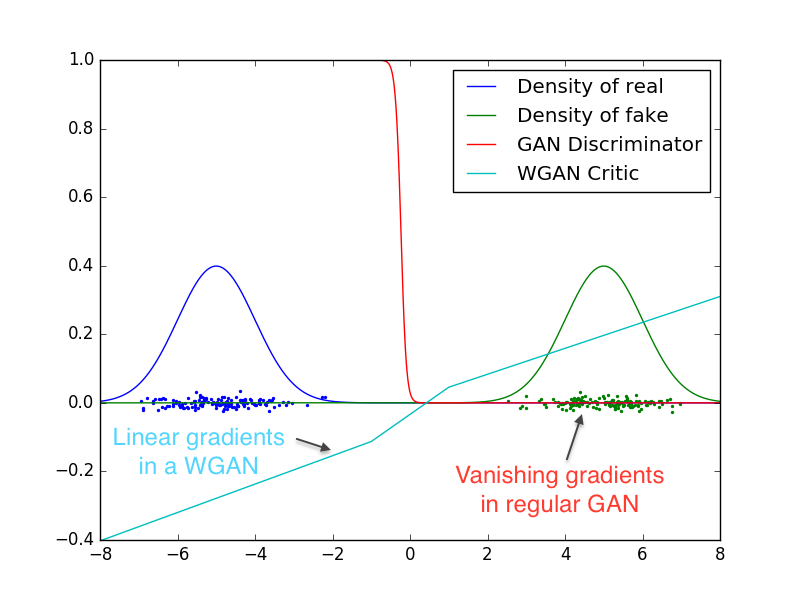
\includegraphics[width=0.9\textwidth]{gan_gradients_gauss.png}
	\end{figure}
\end{frame}

\subsection{Short history of training GANs}
%------------------------------------------------
\begin{frame}
	\frametitle{Short history of training GANs - July 2014}
	\begin{figure}[h!]
		\centering
		
\includegraphics[width=0.9\textwidth]{original_paper.png}
	\end{figure}
	\begin{exampleblock}{GAN Value function}
	\[
		\min_G \max_D \mathbb{E}_{\bm{x} \sim \mathbb{P}_r} \left[ \log D(\bm{x}) \right] + \mathbb{E}_{\bm{z} \sim \mathcal{Z}} \left[ \log (1 -  D(G(\bm{z})))  \right] 
	\]
	\end{exampleblock}
	\begin{itemize}
		\item Discriminator output is probability of image being real (1) or fake (0)
	\end{itemize}
\end{frame}

%------------------------------------------------
\begin{frame}
	\frametitle{Short history of training GANs}
	\begin{itemize}
		\item For G fixed, the optimal discriminator $D^*$ is:
	\end{itemize}
	\[
		D_G^*(\bm{x}) = \frac{p_r(\bm{x})}{p_r(\bm{x}) + p_g(\bm{x})}
	\]
	\pause
	\begin{itemize}
		\item Under an optimal discriminator, generator minimizes the JS-divergence 
	\end{itemize}
	\[
		JS(\mathbb{P}_r \vert \vert \mathbb{P}_g) &= \frac{1}{2}KL\left(\mathbb{P}_r \left|\left|\frac{\mathbb{P}_r + \mathbb{P}_g}{2}\right) + \frac{1}{2}KL\left(\mathbb{P}_g \left| \left| \frac{\mathbb{P}_r + \mathbb{P}_g}{2}\right)
	\]
	\begin{itemize}[<+(1)->]
		\item We want the discriminator (cost function) to be as good as possible
		\item With JS-divergence good discriminator leads to vanishing gradients
		\item Disciminator should be good but not too good?
		\item Bag of tricks 
	\end{itemize}
	\newline
\end{frame}
\subsection{Tricks for training GANs}
%------------------------------------------------
\begin{frame}
	\frametitle{Trick - adding noise}
	\begin{figure}[h!]
		\centering
		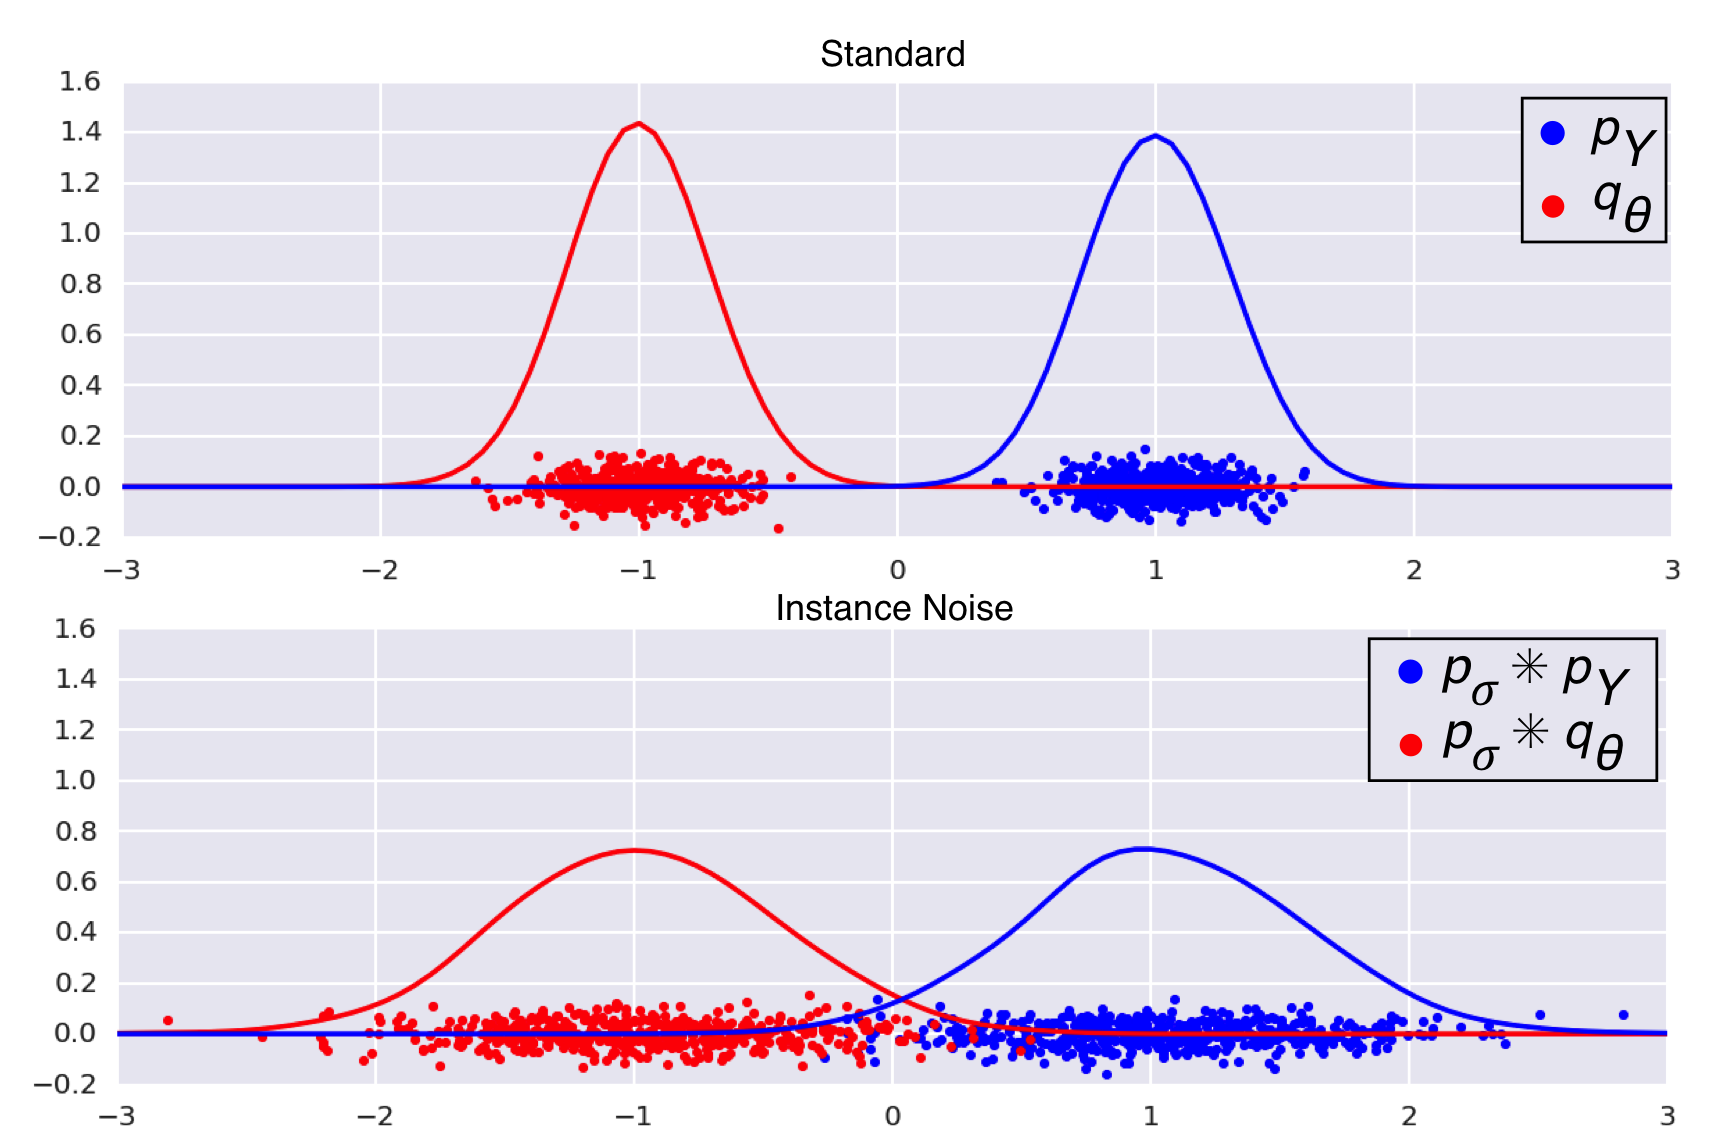
\includegraphics[width=0.8\textwidth]{instance_noise.png}
	\end{figure}
	\begin{itemize}
		\item Matching the noise corresponds to matching the underlying distributions
	\end{itemize}
		\footnotetext{\url{http://www.inference.vc/instance-noise-a-trick-for-stabilising-gan-training/}}
\end{frame}
%------------------------------------------------
\begin{frame}
	\frametitle{Trick - cherrypicking architecture}
		\begin{figure}[h!]
			\centering
			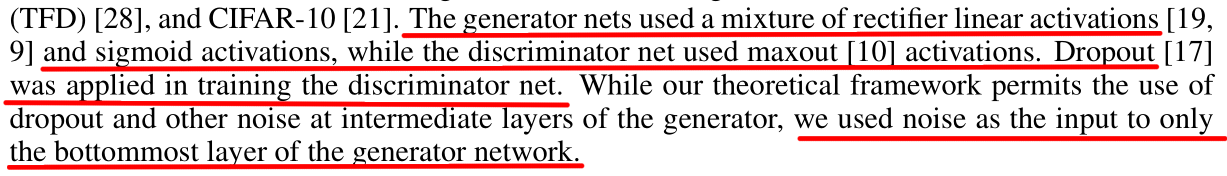
\includegraphics[width=\textwidth]{original_GAN_guidelines.png}
		\end{figure}
		\pause
		\begin{figure}[h!]
			\centering
			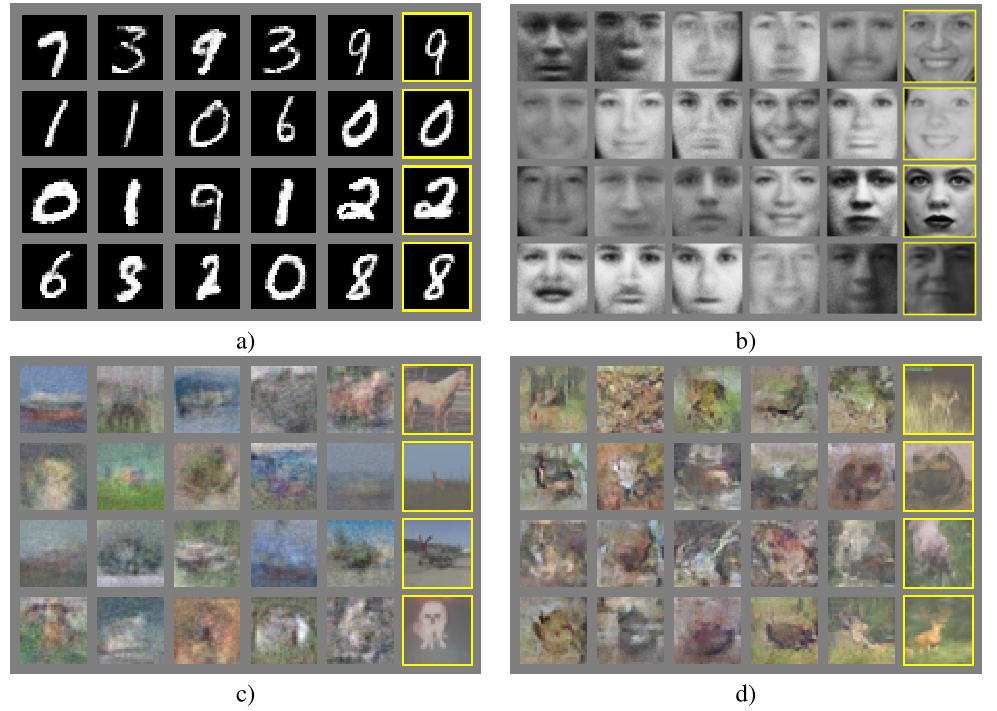
\includegraphics[width=0.65\textwidth]{original_GAN_results.png}
		\end{figure}
\end{frame}
\begin{frame}
	\frametitle{Trick - cherrypicking architecture - DCGAN}
	\begin{figure}[h!]
		\centering
		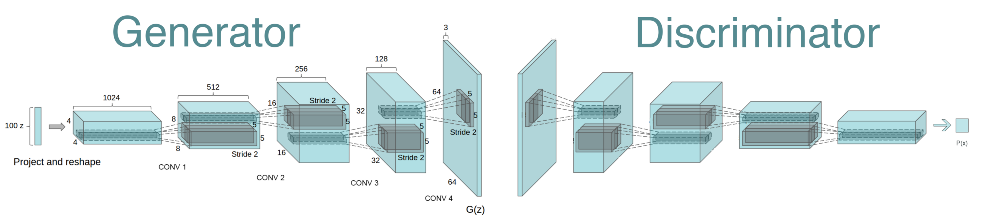
\includegraphics[width=\textwidth]{dcgan_both.png}
	\end{figure}
	\pause
	\begin{figure}[h!]
		\centering
		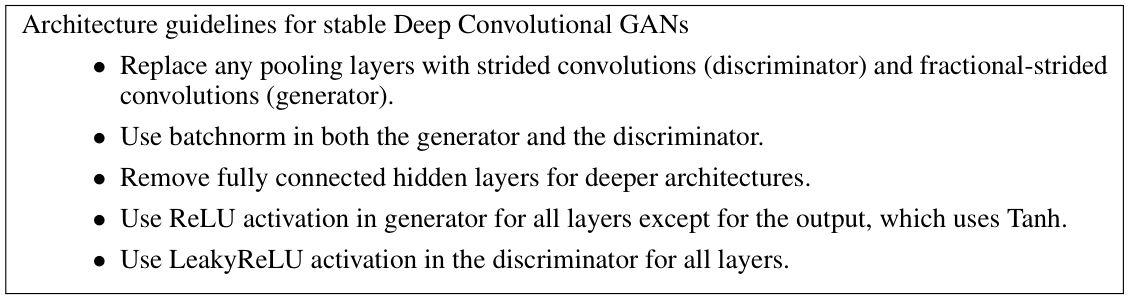
\includegraphics[width=0.8\textwidth]{gan_guidelines.png}
	\end{figure}
	\pause
	\begin{itemize}[<+(1)->]
		\item Chintala reports that they had model generator \footnotemark
		\item No explanation for model performance
		\item Very unstable
	\end{itemize}
	\footnotetext{https://www.youtube.com/watch?v=X1mUN6dD8uE&t=795s}
\end{frame}
%------------------------------------------------
\begin{frame}
	\frametitle{Trick - not training the discriminator until convergence}
	\begin{itemize}[<+->]
		\item Making sure the discriminator is not "too far ahead of" the generator
		\item Each step trains the generator once and discriminator once
		\item Many alternative training plans with questionable efficiency
		\item Has a nice side effect of speeding up the training time
	\end{itemize}
\end{frame}
%------------------------------------------------
\begin{frame}
	\frametitle{But there's a bigger problem...}
	\begin{itemize}
		\item \textbf{Value of the loss doesn't tell us anything!}
		\item No correlation between loss and image quality
		\item Problem stems from mentioned undesired properties of JS-divergence
	\end{itemize}
\end{frame}
%------------------------------------------------
\begin{frame}
	\frametitle{Short history of training GANs}
	\begin{exampleblock}{EM distance}
	\[
		W(\mathbb{P}_r, \mathbb{P}_g) = \inf_{\gamma \in \Pi(\mathbb{P}_r, \mathbb{P}_g)} {\mathbb{E}_{(x, y) \sim \gamma}} \left[ \lvert \lvert x - y \lvert \lvert \right]
	\]
	\end{exampleblock}
	\begin{itemize}[<+(1)->]
		\item How to compute the infimum?
		\item 1000 page book on Optimal Transport \footnotemark
		\item Kantorovich-Rubinstein duality
	\end{itemize}
	\pause
	\begin{exampleblock}{Kantorovich-Rubinstein duality}
	\[
		K \cdot W(\mathbb{P}_r, \mathbb{P}_g) = \sup_{\Vert f \Vert_L \leq K} \mathbb{E}_{x \sim \mathbb{P}_r} \left[ f(x) \right] - \mathbb{E}_{x \sim \mathbb{P}_g} \left[ f(x) \right]
	\]
	\end{exampleblock}
	\pause
	\begin{itemize}
		\item Supremum is the norm over all K-Lipschitz functions $f: \mathcal{X} \rightarrow \mathbb{R} $
	\end{itemize}
	\footnotetext{\url{http://cedricvillani.org/wp-content/uploads/2012/08/preprint-1.pdf}}
\end{frame}

%------------------------------------------------
\begin{frame}
	\frametitle{Lipschitz continuity}
	\begin{exampleblock}{K-Lipschitz function}
	\[
		\vert f(x_1) - f(x_2) \vert \leq K \cdot \vert x_1 - x_2 \vert, \quad \quad \quad \forall x_1, x_2
	\]
	\end{exampleblock}
	\begin{itemize}
		\item Continuous function which is limited how fast it can change
		\item Every function that has a bounded first derivative is Lipschitz
	\end{itemize}
	\begin{figure}[h!]
		\centering
		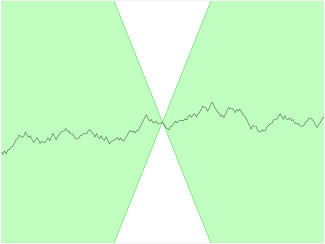
\includegraphics[width=0.5\textwidth]{lipschitz_continuity.png}
	\end{figure}

	\footnotetext{\url{https://en.wikipedia.org/wiki/Lipschitz_continuity}}
\end{frame}

%------------------------------------------------

\begin{frame}
	\frametitle{Short history of training GANs - January 2017}
	\begin{figure}[h!]
		\centering
		
\includegraphics[width=0.9\textwidth]{wgan_paper.png}
	\end{figure}
	\begin{exampleblock}{WGAN Value function}
	\[
		\min_G \max_{D \in \mathcal{D}} \mathbb{E}_{\bm{x} \sim \mathbb{P}_r} \left[ D(\bm{x}) \right] - \mathbb{E}_{\bm{z} \sim \mathcal{Z}} \left[ D(G(\bm{z}))  \right]
	\]
	\begin{center}
		$\mathcal{D}$ - set of all K-Lipschitz functions
	\end{center}
	\end{exampleblock}
	\pause
	\begin{itemize}
		\item Open question - how to effectively enforce the Lipschitz constraint?
	\end{itemize}
\end{frame}

%------------------------------------------------
\begin{frame}
	\frametitle{Method \#1 - Weight Clipping}
	\begin{itemize}[<+->]
		\item After optimization step, clip all weights to $ \big[{-c}, c \big] $
		\item Results in critic being a subset of K-Lipschitz functions, where K is a function of c and the critic's architecture
	\end{itemize}
	\pause
	\begin{figure}[h!]
		\centering
		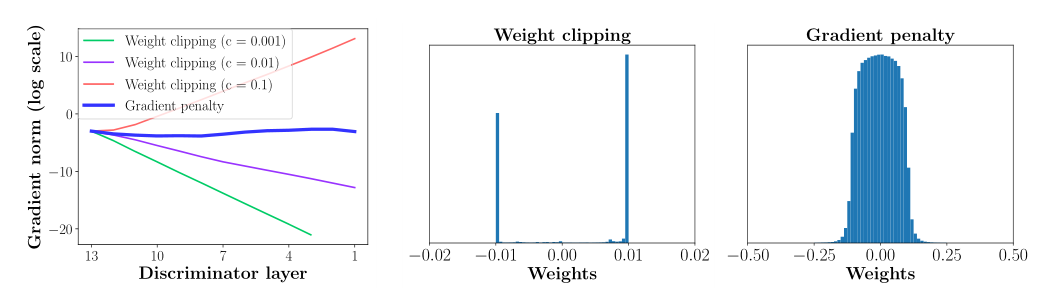
\includegraphics[width=0.9\textwidth]{wgan_clipping_vs_norm.png}
	\end{figure}
	\begin{itemize}[<+->]
		\item Works! But...
		\item Capacity underuse
		\item Exploding and vanishing gradients
	\end{itemize}
\end{frame}
%------------------------------------------------
\begin{frame}
	\frametitle{Method \#2 - Gradient Penalty}
	\begin{columns}
	\begin{column}{0.5\textwidth}
		\begin{itemize}[<+->]
			\item Property of the optimal WGAN critic $ \vert f(x) - f(y) \vert \leq \vert x - y \vert $
			\item Optimal WGAN critic has gradient norm 1
			\item Add a regularization term to the WGAN value function
			\item Sampling along straight lines
		\end{itemize}
		\pause[4]
		\begin{gathered}
			\quad \quad \epsilon \sim U\big[0, 1 \big], \bm{x} \sim \mathbb{P}_g, \bm{\tilde{x}} \sim \mathbb{P}_r \\
			\\

		\quad \bm{\hat{x}} = t \bm{x} + \left( 1 - t \right) \bm{\tilde{x}}

		\end{gathered}
		\pause
		\begin{itemize}
			\item Gradient penalty
		\end{itemize}
		\begin{equation*}
			\onslide<8->{\mathbb{E}_{\bm{\hat{x}} \sim \mathbb{P}_{\bm{\hat{x}}}} \left[ \left(} \onslide<7->{\Vert} \onslide<6->{\nabla_{\bm{\hat{x}}}} D(\bm{\hat{x}}) \onslide<7->{\Vert_2}  \onslide<8->{ - 1 \right)^2  \right]}
		\end{equation*}
	\end{column}
	\pause[5]
	\begin{column}{0.5\textwidth}  %%<--- here
		\begin{figure}[h!]
			\centering
			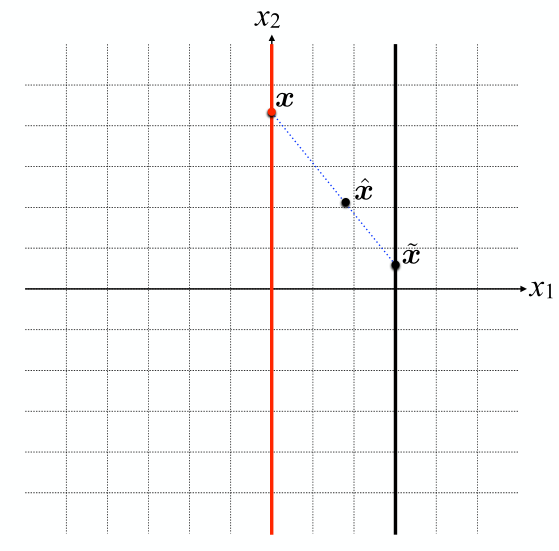
\includegraphics[width=\textwidth]{sampling_x.png}
		\end{figure}
	\end{column}
	\end{columns}
\end{frame}

%------------------------------------------------
\begin{frame}
	\frametitle{Short history of training GANs - March 2017}
	\begin{figure}[h!]
		\centering
		
\includegraphics[width=0.8\textwidth]{wgan_gp_paper.png}
	\end{figure}
	\begin{exampleblock}{WGAN-GP Value function}
	\begin{gather*}
		\min_G \max_{D}
		\mathbb{E}_{\bm{x} \sim \mathbb{P}_r} \Left[ D(\bm{x}) \Right]
		- \mathbb{E}_{\bm{z} \sim \mathcal{Z}} \Left[ D(G(\bm{z}))  \Right] 
		\onslide<2->{+ \lambda \mathbb{E}_{\bm{\hat{x}} \sim \mathbb{P}_{\bm{\hat{x}}}} \left[ \left( \Vert \nabla_{\bm{\hat{x}}} D(\bm{\hat{x}}) \Vert_2  - 1 \right)^2  \right]}
	\end{gather*}
	\end{exampleblock}
	\begin{itemize}[<+(1)->]
		\item Enforcing the Lipschitz constraint with a gradient penalty regularization term
		\item Improvements?
	\end{itemize}
\end{frame}

%------------------------------------------------

\begin{frame}
	\frametitle{Recap}
	\begin{figure}[h!]
	\centering
	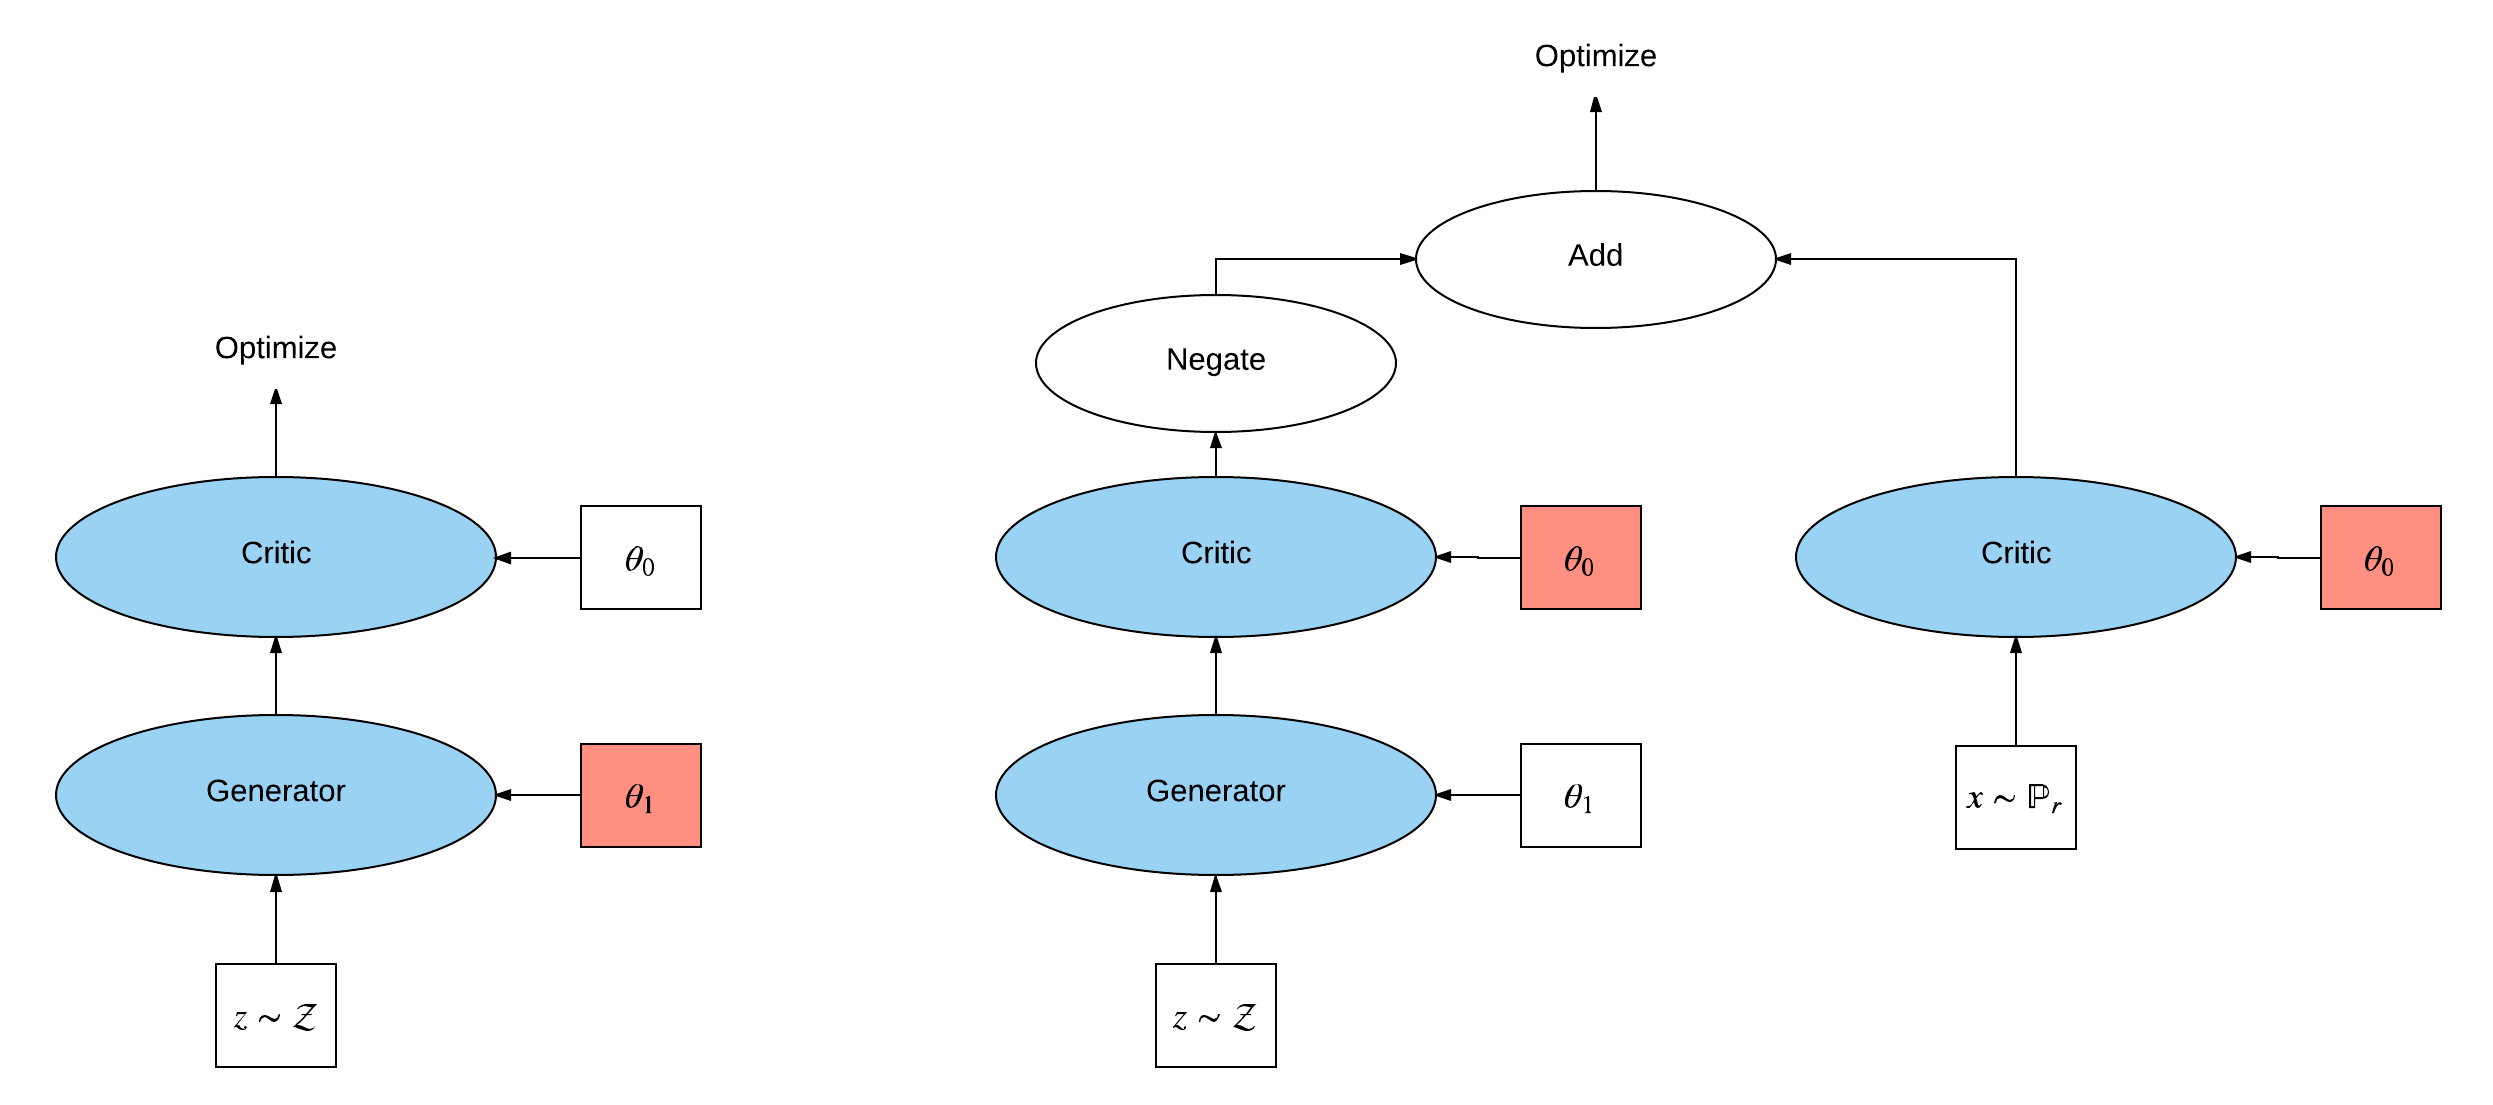
\includegraphics[width=\textwidth]{GAN_optimization_two_step.png}
	\end{figure}
	\begin{itemize}
		\item Using EM distance instead of JS-divergence leads to robust models
		\item Theoretical and empirical data
		\item No need for tricks 
	\end{itemize}
\end{frame}

%------------------------------------------------
\begin{frame}
	\frametitle{Meaningful loss function}
	\begin{figure}[h!]
		\centering
		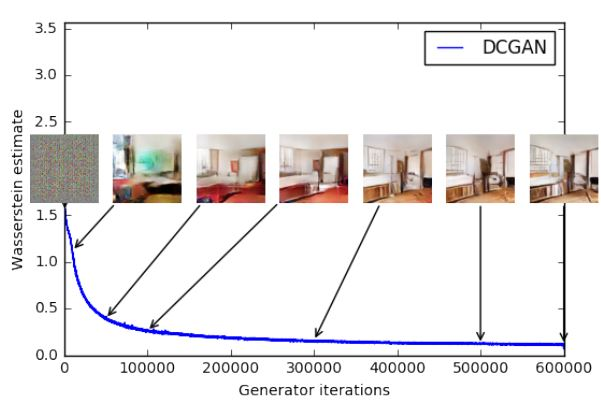
\includegraphics[width=\textwidth]{wgan_loss.jpg}
	\end{figure}
\end{frame}

%------------------------------------------------
\begin{frame} \frametitle{WGAN-GP results}
	\begin{figure}[h!]
	\centering
	\includegraphics<1>[width=\textwidth]{wgan_gp_results_1.png}
	\includegraphics<2>[width=\textwidth]{wgan_gp_results_2.png}
	\end{figure}
\end{frame}
%------------------------------------------------
\begin{frame} \frametitle{WGAN-GP results}
	\begin{figure}[h!]
	\centering
	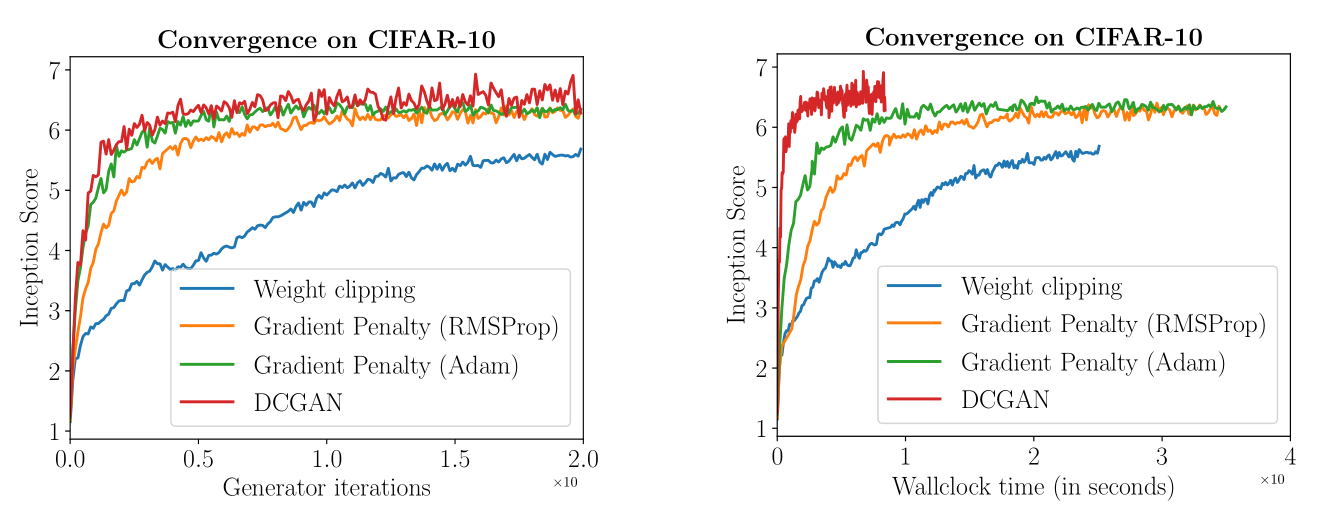
\includegraphics[width=\textwidth]{wgan_gp_graph_results.png}
	\end{figure}
	\begin{itemize}
		\item DCGAN converges faster
		\item Significantly outperforms weight clipping
		\item \textbf{Robust to changes in model architecture}
	\end{itemize}
\end{frame}
%------------------------------------------------

\section{Game theory perspective}
%------------------------------------------------
\begin{frame}
	\frametitle{Game theory perspective}
	\begin{itemize}[<+->]
		\item Two neural networks are playing a zero-sum game
		\item Nash equilibrium
		\item Goal - both players adopting strategies where any deviations would be disadvantageous
		\item Lack of theoretical insights
	\end{itemize}
\end{frame}


\section{GANs - cool stuff}
%------------------------------------------------
\begin{frame}
	\begin{center}
	\Huge{Cool things you can do with GANs}
	\end{center}
\end{frame}

%------------------------------------------------

\begin{frame}
	\frametitle{Latent space arithmetic}
	\begin{figure}[h!]
	\centering
	\includegraphics<1>[width=\textwidth]{vector_space_arithmetic.png}
	\includegraphics<2>[width=0.9\textwidth]{vector_space_arithmetic_2.png}
	\end{figure}
\end{frame}
%------------------------------------------------
\begin{frame}
	\frametitle{Interpolation between images}
	\begin{figure}[h!]
	\centering
	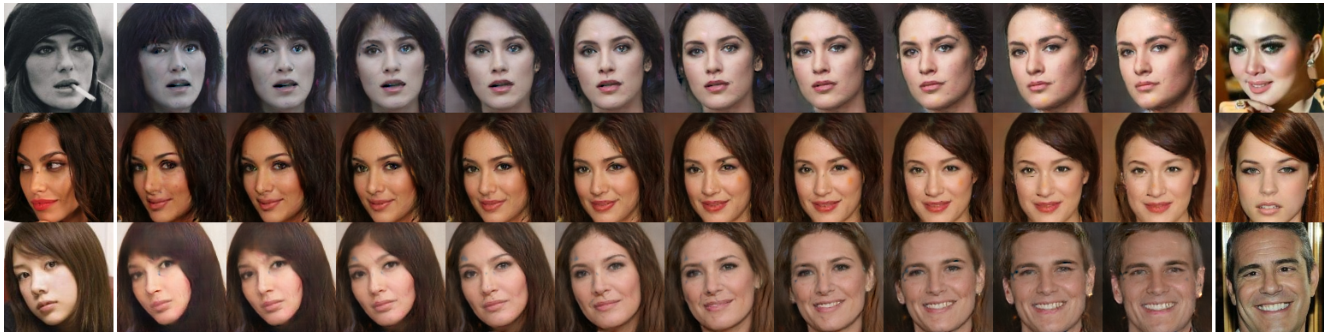
\includegraphics[width=\textwidth]{began_interpolation.png}
	\end{figure}
\end{frame}
%------------------------------------------------
\begin{frame}
	\frametitle{Super-Resolution}
	\begin{figure}[h!]
	\centering
	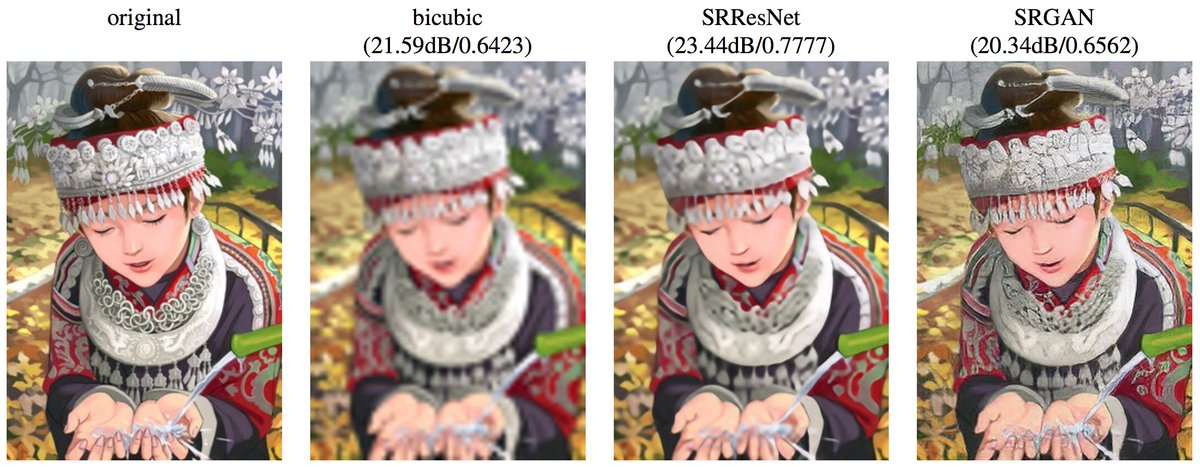
\includegraphics[width=\textwidth]{superresolution.jpg}
	\end{figure}
\end{frame}
%------------------------------------------------
\begin{frame}
	\frametitle{Interactive GAN}
	\begin{figure}[h!]
	\centering
	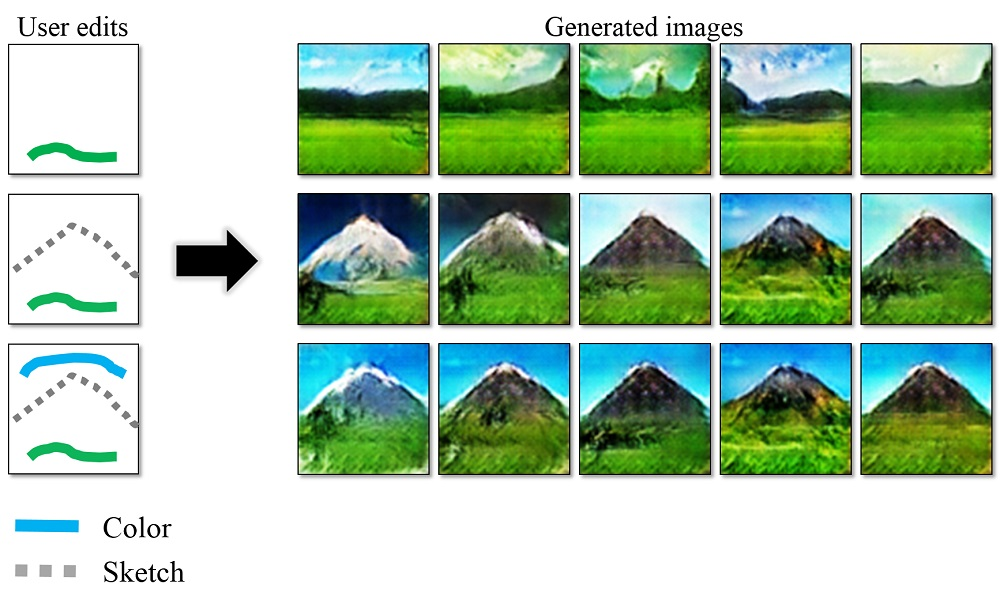
\includegraphics[width=\textwidth]{interactive_gan.jpg}
	\end{figure}
	\href{{https://www.youtube.com/watch?v=9c4z6YsBGQ0}}{\beamergotobutton{Interactive GAN}}
\end{frame}
%------------------------------------------------
\begin{frame}
	\frametitle{Style Transfer}
	\begin{figure}[h!]
	\centering
	\includegraphics<1>[width=\textwidth]{cycle_gan/cg_1.png}
	\includegraphics<2>[width=\textwidth]{cycle_gan/cg_2.png}
	\includegraphics<3>[width=\textwidth]{cycle_gan/cg_3.png}
	\includegraphics<4>[width=\textwidth]{cycle_gan/cg_4.png}
	\includegraphics<5>[width=\textwidth]{cycle_gan/cg_5.png}
	\includegraphics<6>[width=\textwidth]{cycle_gan/cg_6.png}
	\includegraphics<7->[width=\textwidth]{cycle_gan/cyclegan_style_transfer.jpg}
	\end{figure}
	\pause[8]
	\href{https://www.youtube.com/watch?v=9reHvktowLY}{\beamergotobutton{CycleGAN in action}}
	\href{https://twitter.com/quasimondo/status/880005499084734465}{\beamergotobutton{Creepy CycleGAN}}
\end{frame}
%------------------------------------------------
\begin{frame}
	\frametitle{Supervised discriminator}
	\begin{figure}[h!]
	\centering
	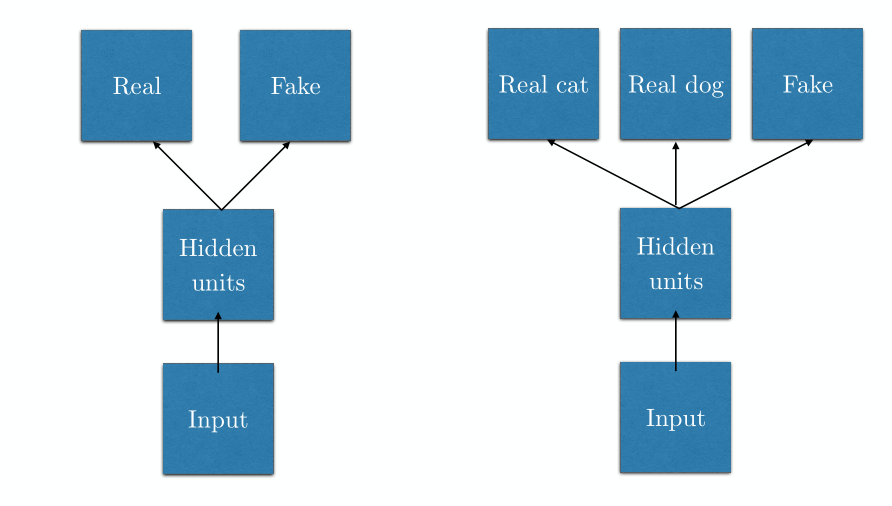
\includegraphics[width=\textwidth]{supervised_discriminator.png}
	\end{figure}
\end{frame}
%------------------------------------------------
\begin{frame}
\frametitle{Heuristics for training WGANs}
\begin{itemize}
	\item Make sure your critic is "ahead of" the generator!
	\item 5-10x more than the generator reduces oscillatory behaviour
	\item Should work without any hyperparameter tuning
\end{itemize}
\end{frame}
%------------------------------------------------
\begin{frame}
\frametitle{Perspectives}
\begin{itemize}
	\item Matching distributions
	\item Neural network as a cost function
	\item Modular training
	\item Two player minimax game
\end{itemize}
\end{frame}

%------------------------------------------------

\section{Problems and open questions}
\begin{frame}
	\frametitle{Problems with GANs}
	\begin{itemize}[<+->]
		\item How to evaluate GANs?
		\item No way to tell how good of an approximation of EM distance the critic really is
		\item Mode collapse
		\item Multi-task solving?
		\item Problems with counting
		\item Perspective
		\item High level structure
		\item Sequential data
	\end{itemize}
\end{frame}
%------------------------------------------------

\begin{frame} \frametitle{Counting}
	\begin{figure}[h!]
	\centering
	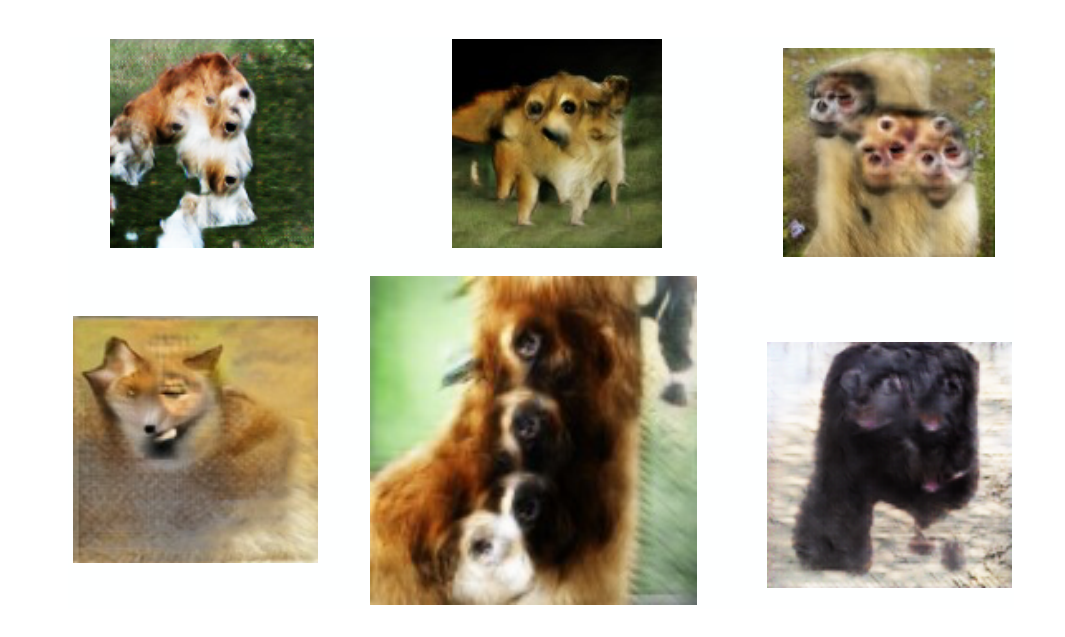
\includegraphics[width=\textwidth]{gan_counting_problem.png}
	\end{figure}
	\footnotetext{Ian J. Goodfellow:
NIPS 2016 Tutorial: Generative Adversarial Networks}
\end{frame}

%------------------------------------------------
\begin{frame} \frametitle{Perspective}
	\begin{figure}[h!]
	\centering
	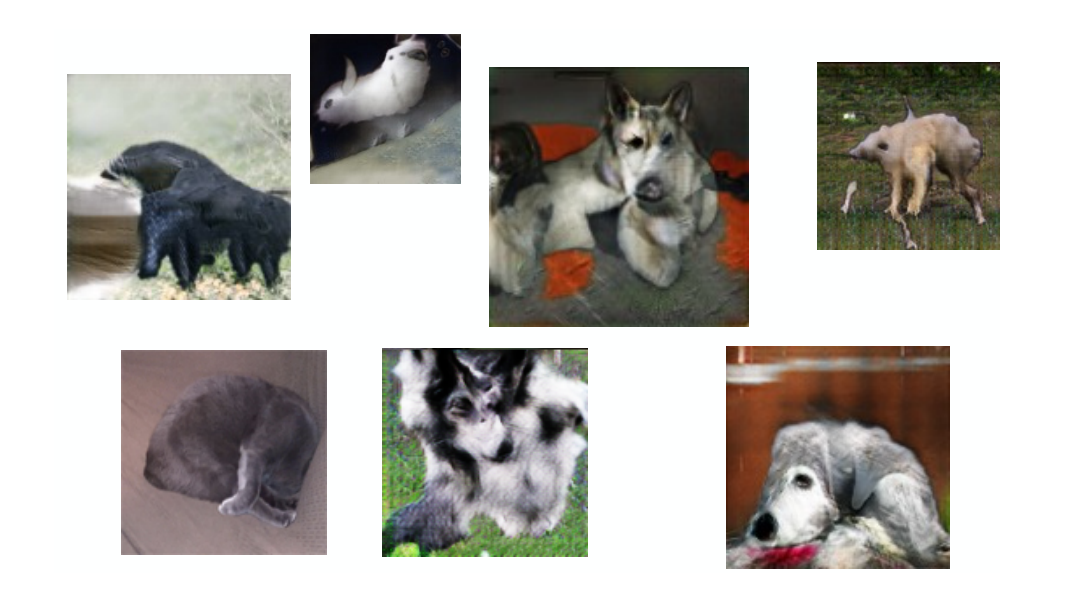
\includegraphics[width=\textwidth]{gan_perspective_problem.png}
	\end{figure}
	\footnotetext{Ian J. Goodfellow:
NIPS 2016 Tutorial: Generative Adversarial Networks}
\end{frame}

%------------------------------------------------
\begin{frame}
	\frametitle{Future of GANs}
	\begin{itemize}[<+->]
		\item Which statistical distance to use?
		\item Best training regime?
		\item Convergence conditions?
		\item Solving mode collapse?
		\item Understanding models with multiple optimization criteria?
	\end{itemize}

	\pause[6]
	\noindent\rule{8cm}{0.4pt}
	\begin{itemize}[<+->]
		\item Sepp Hochreiter - proof of GAN convergence
		\item \textit{Multiplayer} GAN? 
		\item Exchanging discriminators?
		\item Cramer GAN - new statistical distance?
		\item Many, many more papers...
	\end{itemize}
\end{frame}
%------------------------------------------------
\begin{frame}
\frametitle{History of great ideas in deep learning}

\begin{itemize}[<+(1)->]
	\item Need for feature engineering before applying ML model!
	\item \textbf{Oh, neural networks can do that.} Too bad we still have to figure out which cost function to use...
	\item \textbf{Oh, GANs can figure out the cost function by themselves!} Too bad we still have to find the correct way to do the optimization...
	\item \textbf{Oh, the neural network can optimize itself...?}
	\item Learning to learn 
\end{itemize}

\end{frame}

%------------------------------------------------

\begin{frame}
\Huge{\centerline{Thank you!}}
\end{frame}

%----------------------------------------------------------------------------------------

\end{document}
